\chapter{Circuitos electrónicos}

\section{Amplificadores operacionales}

\subsection{Amplificadores diferenciales}

\subsubsection*{El amplificador de instrumentación}

Alguna configuración de amplificador diferencial tiene el inconveniente de que si resistencia de entrada es muy bajita, además de que es complicado configurar una ganancia. El siguiente circuito resuelve el problema:

\begin{figure}[H]
    \centering
    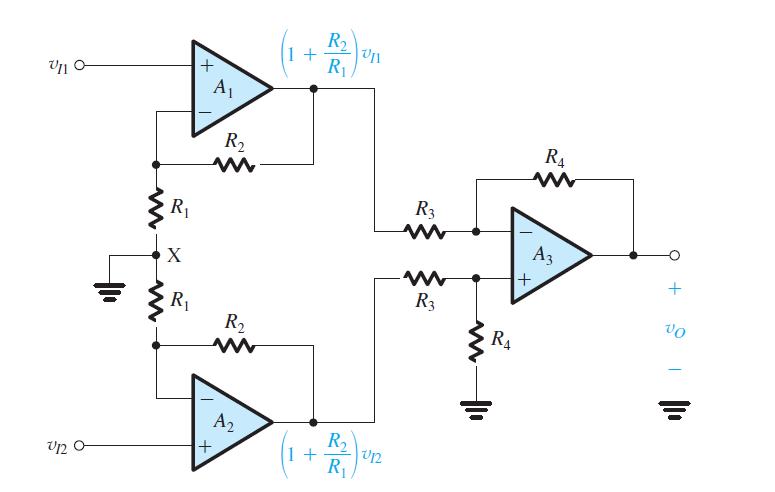
\includegraphics[scale=0.6]{Electronica/electronic_f1.png}
\end{figure}

La salida de la señal está dada por 

\begin{equation*}
\left( \frac{R_4}{R_3} \right) \left( \frac{R_1 + R_2}{R_1} \right) \left( v_{I2} - v_{I1} \right)
\end{equation*}

note que las salidas de las primeras etapas están dadas por $R_1$ y $R_2$, luego se amplifica por $R_3$ y $R_4$. 

Vemos de este circuito dos principales desventajas 

\begin{enumerate}
    \item Los dos amplificadores de la primera etapa deben estar perfectamente sincronizados.
    \item Para variar o configurar la ganancia diferencial, es necesario variar simultáneamente dos resistencias; en la práctica es muy complicado sincronizar el valor de dos resistencia de manera perfecta.
\end{enumerate}

\section{Breve resumen de semiconductores}

En esta sección se tratará muy brevemente y por encima la física y las propiedades de los semiconductores. Todo para introducir los conocimientos necesarios para abordar la física de los diodos y los transistores.

\subsection{Semiconductores intrínsecos}

Como su nombre indica, los semiconductores son materiales cuya conductividad se encuentra entre la de los conductores, como el cobre,, y los aislantes, como el vidrio. Hay dos tipos de semiconductores: semiconductores de un solo elemento como el germanio y el silicio, que se encuentran en el grupo VI de la tabla periódica; y semiconductores compuestos como el arseniuro de galio, que se forman combinando elementos de los grupos III y V o los grupos II y IV. Los semiconductores compuestos son útiles en aplicaciones especiales de circuitos electrónicos, así como en aplicaciones que implican luz, como los diodos emisores de luz. De los dos semiconductores elementales, el germanio se utilizó en la fabricación de los primeros transistores (finales de la década de 1940, principios de la década de 1950). Sin embargo, fue rápidamente reemplazado por el silicio, en el cual se basa casi completamente la tecnología de circuitos integrados de hoy en día. Por esta razón, trataremos principalmente con dispositivos de silicio a lo largo de este libro. Un átomo de silicio tiene cuatro electrones de valencia, por lo que necesita otros cuatro para completar su capa más externa. Esto se logra compartiendo uno de sus electrones de valencia con cada uno de sus cuatro átomos vecinos. Cada par de electrones compartidos forma un enlace covalente. El resultado es que un cristal de silicio puro o intrínseco tiene una estructura de retícula regular, donde los átomos se mantienen en su posición por los enlaces covalentes. \\

A temperaturas suficientemente bajas, cercanas al cero absoluto (0 K), todos los enlaces covalentes permanecen intactos y no hay electrones disponibles para conducir la corriente eléctrica. Por lo tanto, el cristal de silicio intrínseco actúa como un aislante a estas temperaturas.
Sin embargo, a temperatura ambiente, existe suficiente energía térmica para romper algunos de los enlaces covalentes, un proceso conocido como generación térmica. Cuando se rompe un enlace covalente, se libera un electrón, que puede alejarse de su átomo original y conducir la corriente eléctrica si se aplica un campo eléctrico al cristal.
Al alejarse, el electrón deja detrás una carga positiva neta, a la que puede ser atraído un electrón de un átomo vecino, dejando a su vez un "hueco" en su lugar. Este proceso puede repetirse, creando una especie de portador de carga positiva, o hueco, que se mueve por la estructura del cristal de silicio y también puede conducir la corriente eléctrica.
A medida que aumenta la temperatura, se rompen más enlaces covalentes y se generan más pares de electrones y huecos. El incremento en el número de electrones libres y huecos resulta en un aumento en la conductividad del silicio.

La generación térmica resulta en electrones libres y huecos en igual número y, por lo tanto, en igual concentración, donde la concentración se refiere al número de portadores de carga por unidad de volumen (cm3). Los electrones libres y los huecos se mueven aleatoriamente a través de la estructura cristalina del silicio, y en el proceso, algunos electrones pueden llenar algunos de los huecos. Este proceso, llamado recombinación, resulta en la desaparición de electrones libres y huecos. La tasa de recombinación es proporcional al número de electrones libres y huecos, que a su vez está determinada por la tasa de generación térmica. Esta última es una función fuerte de la temperatura. En equilibrio térmico, la tasa de recombinación es igual a la tasa de generación, y se puede concluir que la concentración de electrones libres n es igual a la concentración de huecos p.

\begin{equation*}
n = p = n_i
\end{equation*}

donde $n_i$ denota el número de electrones libres y huecos en una unidad de volumen ($cm^3$) de silicio intrínseco a una temperatura dada. Los resultados de la física de semiconductores dan $n_i$ como

\begin{equation*}
n_i = BT^{3/2} e^{\frac{-E_g}{2kT}}
\end{equation*}

donde B es un parámetro dependiente del material que es $7.3 \ 10^15 cm^{-3}K^{-3/2}$ para el silicio; $T$ es la temperatura en K; $E_g$, un parámetro conocido como la energía de Fermi, es de $1.12 Ev$ para el silicio; y $k$ es la constante de Boltzmann ($8.62 \ 10^-5 eV/K$). 
Es interesante saber que la energía de la banda prohibida $E_g$ es la energía mínima requerida para romper un enlace covalente y, por lo tanto, generar un par de electrones-huecos.

Finalmente, es útil conocer la relación de portadores y la concentración 

\begin{equation*}
p \ n = n_i^2 
\end{equation*}

Para el silicio a temperatura ambiente, $n_i \approx 1.5 \ 10^{10} cm^{-3}$


\subsection{Semiconductores dopados}

El cristal de silicio intrínseco que se describió anteriormente tiene igual concentración de electrones libres y huecos, generados por la generación térmica. Sin embargo, estas concentraciones son demasiado pequeñas para que el silicio conduzca una corriente apreciable a temperatura ambiente. Además, las concentraciones de portadores y, por ende, la conductividad, son funciones fuertes de la temperatura, lo cual no es una propiedad deseable en un dispositivo electrónico. Afortunadamente, se desarrolló un método para cambiar la concentración de portadores en un cristal semiconductor de forma sustancial y controlada. Este proceso se conoce como dopado, y el silicio resultante se conoce como silicio dopado.

El dopado implica la introducción de átomos de impurezas en el cristal de silicio en cantidades suficientes para aumentar de forma considerable la concentración de electrones libres o huecos, pero con poco o ningún cambio en las propiedades cristalinas del silicio. Para aumentar la concentración de electrones libres, se dopa el silicio con un elemento con una valencia de 5, como el fósforo, y el silicio dopado resultante se conoce como tipo n. Para aumentar la concentración de huecos, se dopa el silicio con un elemento con una valencia de 3, como el boro, y el silicio dopado resultante se conoce como tipo p.

Un ejemplo de esto es un cristal de silicio dopado con fósforo. Los átomos de fósforo reemplazan a algunos de los átomos de silicio en la estructura cristalina. Como el átomo de fósforo tiene cinco electrones en su capa externa, cuatro de estos electrones forman enlaces covalentes con los átomos vecinos, y el quinto electrón se convierte en un electrón libre. Así, cada átomo de fósforo dona un electrón libre al cristal de silicio, y la impureza de fósforo se llama donante. Sin embargo, este proceso no genera huecos. La carga positiva neta asociada con el átomo de fósforo es una carga ligada que no se mueve a través del cristal.

Si la concentración de átomos donantes es ND, donde ND es usualmente mucho mayor que ni, la concentración de electrones libres en el silicio de tipo n será

\begin{equation*}
n_n \approx N_D
\end{equation*}

De la ecuación de portadores se tiene que 

\begin{equation*}
p_n = \frac{n_i^2}{N_D}
\end{equation*}

Así, $p_n$ tendrá la misma dependencia de la temperatura que $n_i^2$. Finalmente, debemos notar que en el silicio de tipo n, la concentración de electrones libres $n_n$ será mucho mayor que la de los huecos. Por lo tanto, se dice que los electrones son los portadores de carga mayoritarios y los huecos los portadores de carga minoritarios en el silicio de tipo n.

Para semiconductores tipo $p$ se tiene concentraciones $N_A \gg n_i$

\begin{equation*}
p_p \approx N_A
\end{equation*}

\begin{equation*}
p_p n_p = n_i^2
\end{equation*}

\begin{equation*}
n_p \approx \frac{n_i^2}{N_A}
\end{equation*}

\subsection{Flujo de corriente en el semiconductor}

Hay dos mecanismos para el movimiento de los portadores de carga: por arrastre y por difusión

\subsubsection{Corriente de arrastre}

cuando hay un campo eléctrico $E$ aplicado en el cristal semiconductor, los huecos son acelerados en la dirección del campo, y los electrones libres en la dirección contraria. Los huecos adquieren entonces una velocidad de arrastre ada por 

\begin{equation*}
v_{p-drift} = \mu_p E
\end{equation*}

Donde el término $\mu_p$ se denomina movilidad de huecos.  Representa la facilidad con la que los huecos se mueven a través del cristal. La movilidad de huecos para los cristales semiconductores de silicio es 

\begin{equation*}
\mu_p = 480 \ \frac{\text{cm}^2}{\text{V s}}
\end{equation*}

La movilidad de los electrones es por su parte 

\begin{equation*}
v_{n-drift} = -\mu_n E
\end{equation*}

\begin{equation*}
\mu_n = 1350 \ \frac{\text{cm}^2}{\text{V s}}
\end{equation*}

\begin{figure}[H]
    \centering
    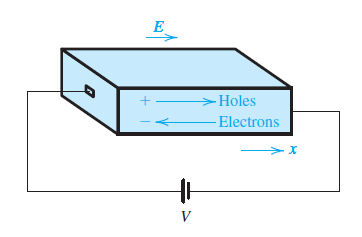
\includegraphics[scale=0.6]{Electronica/semiconductor_f1.png}
\end{figure}

Volviendo al barra de silicio monocristalino mostrada en la última imagen, sea p la concentración de huecos y la de electrones libres sea n. Queremos calcular el componente de corriente debido al flujo de huecos. Consideremos un plano perpendicular a la dirección x. En un segundo, la carga del hueco que cruza ese plano será de ($A q p v_{p-drift}$) culombios, donde A es el área transversal de la barra de silicio y q es la magnitud de la carga del electrón. Esto debe ser el componente del hueco de la corriente de deriva que fluye a través de la barra.

\begin{eqnarray*}
I_P &=& A q p v_{p-drift} \\
I_P &=& A q p \mu_p E
\end{eqnarray*}

La densidad de corriente será entonces

\begin{equation*}
J_p =\frac{I_p}{A} = q p \mu_p E
\end{equation*}

El componente de corriente debido a la deriva de los electrones libres se puede encontrar de manera similar. Sin embargo, debemos notar que los electrones que derivan de derecha a izquierda dan como resultado un componente de corriente de izquierda a derecha. Esto se debe a la convención de tomar la dirección del flujo de corriente como la dirección del flujo de carga positiva y opuesta a la dirección del flujo de carga negativa. Entonces,

\begin{eqnarray*}
I_n &=& -A q n v_{n-drift} \\
J_n &=& q n \mu_n E
\end{eqnarray*}

La dcensidad neta de corriente es

\begin{equation*}
J = J_p + J_n = q (p \mu_o + n \mu_n) E
\end{equation*}

Vemos que esto indica una resistividad (o conductividad) dada por 

\begin{equation*}
\rho = \frac{1}{\sigma} = \frac{1}{q(p \mu_p + n \mu_n)}
\end{equation*}

\subsubsection{Corriente de difusión}

\begin{figure}[H]
    \centering
    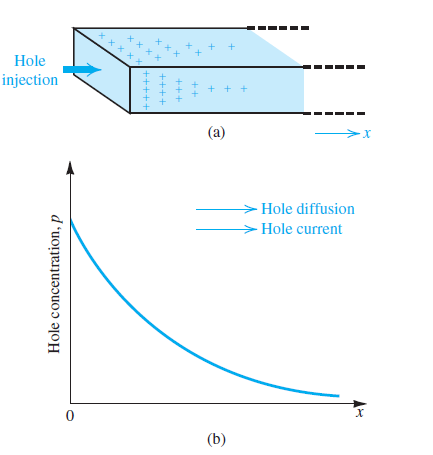
\includegraphics[scale=0.6]{Electronica/semiconductor_f2.png}
\end{figure}

La difusión de portadores ocurre cuando la densidad de portadores de carga en un trozo de semiconductor no es uniforme. Por ejemplo, si por algún mecanismo la concentración de huecos es mayor en una parte de un trozo de silicio que en otra, entonces los huecos se difundirán de la región de alta concentración a la región de baja concentración. Este proceso de difusión es similar al que se observa si se dejan caer unas gotas de tinta en un tanque lleno de agua. La difusión de los portadores de carga da lugar a un flujo neto de carga, o corriente de difusión.

Por ejemplo, considera la barra de silicio mostrada en la parte (a) de la figura: por algún proceso no especificado, hemos dispuesto inyectar huecos en su lado izquierdo. Esta inyección continua de huecos da lugar a y mantiene un perfil de concentración de huecos como el que se muestra en la parte (b) de la figura. Este perfil a su vez provoca que los huecos se difundan de izquierda a derecha a lo largo de la barra de silicio, resultando en una corriente de huecos en la dirección x. La magnitud de la corriente en cualquier punto es proporcional a la pendiente del perfil de concentración, o el gradiente de concentración, en ese punto.

\begin{equation*}
J_p = -q D_p \frac{d p(x)}{dx}
\end{equation*}

Donde el término $D_p$ se denomina constante de difusión o difusividad de los huecos, y $p(x)$ es la concentración de huecos en función de $x$.

En el caso de la difusión resultante de un gradiente de concentración de electrones, se tiene que

\begin{equation*}
J_n = q D_n \frac{d n(x)}{dx}
\end{equation*}

Observe que un valor negativo de $(dn/dx)$ da lugar a una corriente negativa, resultado de la convención que establece que la dirección positiva de la corriente se toma como la del flujo de carga positiva (y opuesta a la del flujo de carga negativa). Para huecos y electrones que se difunden en silicio intrínseco, los valores típicos para las constantes de difusión son $Dp = 12 cm2/s$ y $Dn = 35 cm2/s$.

\subsubsection*{Relación entre $\mu$ y $D$}

La siguiente relación entre la difusividad y movilidad puede ser de gran importancia

\begin{equation*}
\frac{D_n}{\mu_n} = \frac{D_p}{\mu_p} = V_T
\end{equation*}

\subsection{La unión PN} \label{subSeccionUnionPN}

\begin{figure}[H]
    \centering
    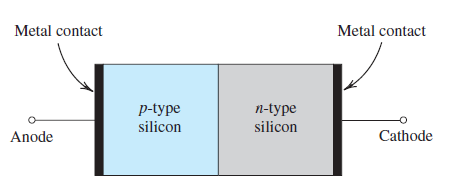
\includegraphics[scale=0.6]{Electronica/pn_f1.png}
\end{figure}

La juntora pn es el implementador del diodo.

\subsubsection{Estructura física}

La figura anterior muestra una estructura física simplificada de la unión pn. Consiste en un semiconductor tipo p (por ejemplo, silicio) en contacto cercano con un material semiconductor tipo n (también silicio). En la práctica, ambas regiones p y n son parte del mismo cristal de silicio; es decir, la unión pn se forma dentro de un solo cristal de silicio creando regiones con diferentes tipos de dopado (regiones p y n). Como se indica en la figura, las conexiones de cables externos se hacen a las regiones p y n a través de contactos de metal (aluminio). Si la unión pn se utiliza como un diodo, estos constituyen los terminales del diodo y por lo tanto se etiquetan como "ánodo" y "cátodo" en consonancia con la terminología de los diodos.

\subsubsection{Operación con las terminales en circuito abierto}

\begin{figure}[H]
    \centering
    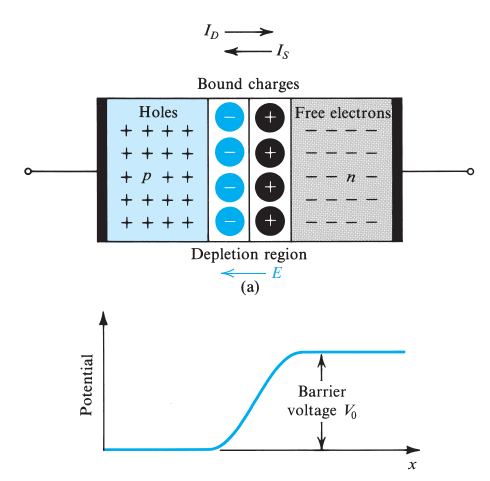
\includegraphics[scale=0.6]{Electronica/pn_f2.png}
\end{figure}

La figura muestra una unión pn en condiciones de circuito abierto, es decir, los terminales externos están desconectados. Los signos "+" en el material tipo p denotan los huecos mayoritarios. La carga de estos huecos es neutralizada por una cantidad igual de carga negativa ligada asociada con los átomos aceptores. Para simplificar, estas cargas ligadas no se muestran en el diagrama. Tampoco se muestran los electrones minoritarios generados en el material tipo p por ionización térmica.

En el material tipo n, los electrones mayoritarios están indicados por signos "-". Aquí también, la carga positiva ligada que neutraliza la carga de los electrones mayoritarios no se muestra para mantener el diagrama simple. El material tipo n también contiene huecos minoritarios generados por ionización térmica, pero no se muestran en el diagrama.

\paragraph*{Corriente de difusión $I_D$} Debido a que la concentración de huecos es alta en la región p y baja en la región n, los huecos se difunden a través de la unión desde el lado p al lado n. De manera similar, los electrones se difunden a través de la unión desde el lado n al lado p. Estas dos componentes de corriente se suman para formar la corriente de difusión $I_D$, cuya dirección es del lado p al lado n, como se indica en la Figura.

\paragraph*{Zona de deplexión}Los huecos que se difunden a través de la unión hacia la región n rápidamente recombinan con algunos de los electrones mayoritarios presentes allí, desapareciendo. Este proceso de recombinación también provoca la desaparición de algunos electrones libres del material tipo n. Por lo tanto, parte de la carga positiva ligada ya no estará neutralizada por electrones libres, y se dice que esta carga ha sido "descubierta". Como la recombinación ocurre cerca de la unión, habrá una zona próxima a la unión que estará desprovista de electrones libres y contendrá carga positiva ligada no cubierta, como se muestra en la figura.

Los electrones que se difunden a través de la unión hacia la región p rápidamente recombinan con algunos de los huecos mayoritarios allí, y por lo tanto desaparecen. Esto también resulta en la desaparición de algunos huecos mayoritarios, haciendo que parte de la carga negativa ligada quede descubierta. Por lo tanto, en el material p cerca de la unión, habrá una región sin huecos y con carga negativa ligada no cubierta, como se indica en la figura.

A partir de lo anterior, se deduce que existirá una región de agotamiento de portadores a ambos lados de la unión, con el lado n cargado positivamente y el lado p cargado negativamente. Esta región de agotamiento, o simplemente región de deplexión, también se llama región de carga espacial. Las cargas en ambos lados de la región de deplexión generan un campo eléctrico \(E\) a través de la región, como se indica en la figura. Por lo tanto, se produce una diferencia de potencial a través de la región de deplexión, con el lado n a una tensión positiva en relación con el lado p, como se muestra en la figura. Así, el campo eléctrico resultante se opone a la difusión de huecos hacia la región n y de electrones hacia la región p. De hecho, la caída de tensión a través de la región de deplexión actúa como una barrera que debe superarse para que los huecos se difundan hacia la región n y los electrones hacia la región p. Cuanto mayor sea el voltaje de barrera, menor será el número de portadores que podrán superar la barrera y, por lo tanto, menor será la magnitud de la corriente de difusión. Por lo tanto, es la aparición del voltaje de barrera \(V_0\) lo que limita el proceso de difusión de portadores. De ello se deduce que la corriente de difusión \(I_D\) depende fuertemente de la caída de tensión \(V_0\) a través de la región de deplexión.

\paragraph*{Corriente de arrastre $I_s$ y equilibrio} Además del componente de corriente $I_D$ debido a la difusión de portadores mayoritarios, existe un componente debido a la deriva de portadores minoritarios en la unión. Específicamente, algunos de los huecos generados térmicamente en el material n se mueven hacia la unión y alcanzan el borde de la región de agotamiento. Allí, experimentan el campo eléctrico en la región de agotamiento, que los arrastra a través de esa región hacia el lado p. De manera similar, algunos de los electrones minoritarios generados térmicamente en el material p se mueven hacia el borde de la región de agotamiento y son arrastrados por el campo eléctrico en la región de agotamiento hacia el lado n. Estos dos componentes de corriente —electrones movidos por deriva de p a n y huecos movidos por deriva de n a p— se suman para formar la corriente de deriva $I_S$, cuya dirección es desde el lado n hacia el lado p de la unión, como se indica en la Fig. 3.9. Dado que la corriente $I_S$ es transportada por portadores minoritarios generados térmicamente, su valor depende fuertemente de la temperatura; sin embargo, es independiente del valor del voltaje V0 en la capa de agotamiento. Esto se debe al hecho de que la corriente de deriva está determinada por el número de portadores minoritarios que llegan al borde de la región de agotamiento; cualquier portador minoritario que logre llegar al borde de la región de agotamiento será arrastrado por E, independientemente del valor de E o, correspondientemente, de V0.
Bajo condiciones de circuito abierto no existe corriente externa; por lo tanto, las dos corrientes opuestas a través de la unión deben ser iguales en magnitud.

\begin{equation*}
I_D = I_S
\end{equation*}

Esta condición de equilibrio es mantenida por el voltaje de barrera $V_0$. Por lo tanto, si por alguna razón $I_D$ excede a $I_S$, entonces se descubrirá más carga ligada en ambos lados de la unión, la capa de agotamiento se ensanchará y el voltaje a través de ella ($V_0$) aumentará. Esto, a su vez, provoca que $I_D$ disminuya hasta que se logre el equilibrio con $I_D= I_S$. Por otro lado, si $I_S$ excede a $I_D$, entonces la cantidad de carga descubierta disminuirá, la capa de agotamiento se estrechará y el voltaje a través de ella ($V_0$) disminuirá. Esto hace que $I_D$ aumente hasta que se logre el equilibrio con $I_D$ = $I_S$.

\subsubsection{Voltaje Incorporado en la Unión} Sin voltaje externo aplicado, se puede demostrar que el voltaje de barrera V0 a través de la unión pn está dado por

\begin{equation*}
V_0 = V_T \ln{\left(\frac{N_A N_D}{n_i^2}\right)}
\end{equation*}

donde \(N_A\) y \(N_D\) son las concentraciones de dopaje del lado p y del lado n de la unión, respectivamente. Por lo tanto, \(V_0\) depende tanto de las concentraciones de dopaje como de la temperatura. Es conocido como el voltaje incorporado en la unión. Típicamente, para el silicio a temperatura ambiente, \(V_0\) está en el rango de 0,6 V a 0,9 V.

Cuando los terminales de la unión pn se dejan en circuito abierto, el voltaje medido entre ellos será cero. Es decir, el voltaje \(V_0\) a través de la región de agotamiento no aparece entre los terminales de la unión. Esto se debe a los voltajes de contacto existentes en las uniones metal-semiconductor en los terminales, que contrarrestan y equilibran exactamente el voltaje de barrera. Si no fuera así, habríamos podido extraer energía de la unión pn aislada, lo que claramente violaría el principio de conservación de la energía.

\paragraph*{Ancho y Carga Almacenada en la Región de Agotamiento} La figura siguiente proporciona una ilustración adicional de la situación que prevalece en la unión pn cuando la unión está en equilibrio. En la figura(a) mostramos una unión en la cual \(N_A > N_D\), una situación típica en la práctica. Esto se confirma por la concentración de portadores en ambos lados de la unión, como se muestra en la figura(b). Observe que hemos denotado las concentraciones de portadores minoritarios en ambos lados por \(n_{p0}\) y \(p_{n0}\), con el subíndice adicional "0" significando equilibrio (es decir, antes de que se apliquen voltajes externos, como se verá en la siguiente sección). 

\begin{figure}[H]
    \centering
    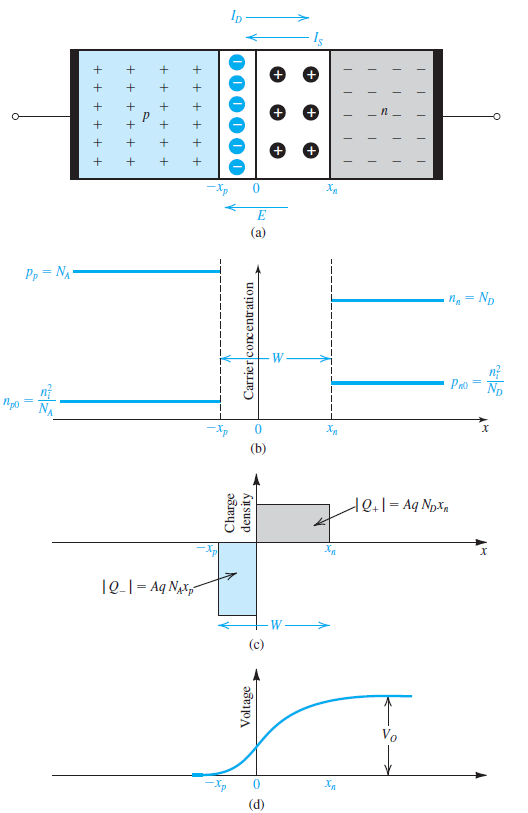
\includegraphics[scale=0.6]{Electronica/pn_f3.png}
\end{figure}

Observe que la región de agotamiento se extiende en los materiales p y n y que existen cantidades iguales de carga en ambos lados ($Q_+$ y $Q_-$ en la figura(c)). Sin embargo, ya que usualmente se utilizan dopajes desiguales \(N_A\) y \(N_D\), como en el caso ilustrado en la figura, el ancho de la capa de agotamiento no será el mismo en los dos lados. Más bien, para descubrir la misma cantidad de carga, la capa de agotamiento se extenderá más profundamente en el material menos dopado. Específicamente, si denotamos el ancho de la región de agotamiento en el lado p por \(x_p\) y en el lado n por \(x_n\), podemos expresar la magnitud de la carga en el lado n de la unión como: 

\begin{eqnarray*}
|Q_+| = q A x_n N_D \\
|Q_-| = q A x_p N_A 
\end{eqnarray*}

donde \(A\) es el área de la sección transversal de la unión en el plano perpendicular a la página. La condición de igualdad de carga ahora puede escribirse como:

\begin{equation*}
q A x_n N_D = q A x_p N_A
\end{equation*}

\begin{equation*}
\frac{x_n}{x_p} = \frac{N_A}{N_D}
\end{equation*}

En la práctica real, es común que un lado de la unión esté mucho más dopado que el otro, con el resultado de que la región de agotamiento existe casi enteramente en un lado (el lado ligeramente dopado).

El ancho \(W\) de la capa de agotamiento se puede demostrar que está dado por:

\begin{equation}
W = x_n + x_p = \sqrt{\frac{2 \epsilon_s}{q}\left( \frac{1}{N_A} + \frac{1}{N_D} \right) V_0}
\label{eq_anchoZonaDeplexion}
\end{equation}

donde \( \epsilon_s \) es la permitividad eléctrica del silicio \( = 11.7 \epsilon_0 \)
\( 11.7 \times 8.85 \times 10^{-14} \) F/cm \( = 1.04 \ 10^{-12} \) F/cm. Típicamente, \( W \) está en el rango de $0.1 \mu m$ a $1 \mu m$. Las ecuaciones anteriores se pueden usar para obtener \( xn \) y \( xp \) en términos de \( W \) como:

\begin{eqnarray*}
x_n &=& W \frac{N_A}{N_A + N_D} \\
x_n &=& W \frac{N_D}{N_A + N_D}
\end{eqnarray*}

La carga almacenada en cualquiera de los lados de la región de agotamiento se puede expresar en términos de \( W \) utilizando las ecuaciones anteriores para obtener:

\begin{eqnarray*}
Q_J = |Q_+| = |Q_-| \\
Q_J = A q \left( \frac{N_A N_D}{N_A + N_D} \right)
\end{eqnarray*}

Finalmente, podemos sustituir por \( W \) de la Ec. (3.26) para obtener:

\begin{equation*}
Q_J = A \sqrt{2 \epsilon_s q \left( \frac{N_A N_D}{N_A + N_D} \right)V_0}
\end{equation*}

Estas expresiones para \( Q_J \) serán útiles en las siguientes secciones.

\subsubsection{La unión pn bajo una tensión aplicada}

Después de haber estudiado en detalle la unión pn en circuito abierto, ahora estamos listos para aplicar un voltaje de corriente continua entre sus dos terminales para descubrir sus propiedades de conducción eléctrica. Si se aplica el voltaje de manera que el lado p se haga más positivo que el lado n, se le conoce como voltaje con polarización directa (o forward-bias). Por el contrario, si nuestro voltaje de corriente continua aplicado hace que el lado n sea más positivo que el lado p, se dice que tiene una polarización inversa (o reverse-bias). Como veremos, la unión pn muestra propiedades de conducción extremadamente diferentes en sus direcciones directa e inversa.

\paragraph*{Descripción cualitativa de la operación de unión}


La figura muestra la unión pn bajo tres condiciones diferentes: (a) la condición de circuito abierto o equilibrio estudiada en la sección anterior; (b) la condición de polarización inversa, donde se aplica un voltaje de corriente continua \(V_R\); y (c) la condición de polarización directa, donde se aplica un voltaje de corriente continua \(V_F\). Observe que en el caso de circuito abierto, se desarrolla un voltaje de barrera \(V_0\), haciendo que n sea más positivo que p, y limitando la corriente de difusión \(I_D\) a un valor exactamente igual a la corriente de deriva \(I_S\), dando como resultado una corriente cero en los terminales de la unión, como debería ser el caso, ya que los terminales están en circuito abierto. Además, como se mencionó anteriormente, el voltaje de barrera \(V_0\), aunque establece el equilibrio de corriente a través de la unión, en realidad no aparece entre los terminales de la unión.

\begin{figure}[H]
    \centering
    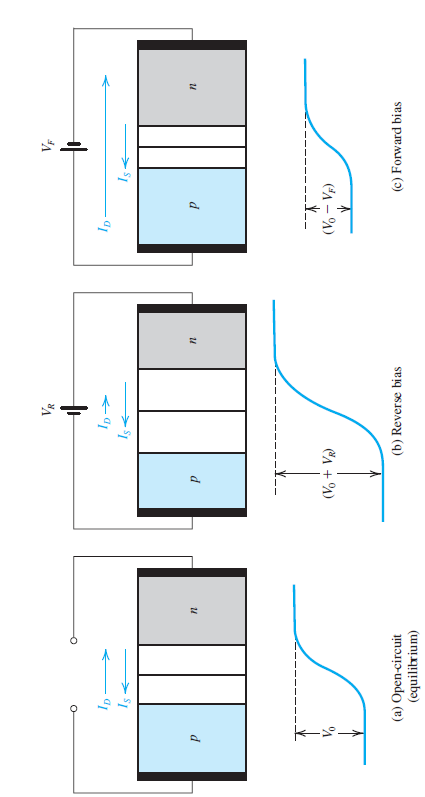
\includegraphics[scale=0.6,angle=-90]{Electronica/pn_f4.png}
\end{figure}

Consideremos ahora el caso de polarización inversa en (b). El voltaje de polarización inversa externamente aplicado \(V_R\) va en la dirección para sumar al voltaje de barrera, y lo hace, aumentando así el voltaje de barrera efectivo a \(V_0 + V_R\) como se muestra. Esto reduce el número de huecos que difunden en la región n y el número de electrones que difunden en la región p. El resultado final es que la corriente de difusión \(I_D\) se reduce drásticamente. Como veremos en breve, un voltaje de polarización inversa de un voltio o algo así es suficiente para hacer que \(I_D \approx 0\), y la corriente a través de la unión y a través del circuito externo será igual a \(I_S\). Recordando que \(I_S\) es la corriente debida a la deriva a través de la región de agotamiento de los portadores minoritarios generados térmicamente, esperamos que \(I_S\) sea muy pequeño y que dependa fuertemente de la temperatura. Demostraremos que este es el caso muy pronto. Llegamos así a la conclusión de que en la dirección inversa, la unión pn conduce una corriente muy pequeña y casi constante igual a \(I_S\).

Antes de abandonar el caso de polarización inversa, observe que el aumento del voltaje de barrera irá acompañado de un aumento correspondiente de la carga almacenada no neutralizada en ambos lados de la región de agotamiento. Esto a su vez significa una región de agotamiento más amplia, necesaria para descubrir la carga adicional requerida para soportar el mayor voltaje de barrera \(V_0 + V_R\). Analíticamente, estos resultados pueden obtenerse fácilmente mediante una simple extensión de los resultados del caso de equilibrio. Por lo tanto, el ancho de la región de agotamiento se puede obtener reemplazando \(V_0\) en la ecuación \ref{eq_anchoZonaDeplexion} por \(V_0 + V_R\). De manera similar será para la carga almacenada.

A continuación, consideramos el caso de polarización directa mostrado en la figura (c). Aquí el voltaje aplicado \(V_F\) está en la dirección que resta del voltaje incorporado \(V_0\), resultando en un voltaje de barrera reducido (\(V_0 - V_F\)) a través de la región de agotamiento. Este voltaje de barrera reducido irá acompañado de una carga reducida en la región de agotamiento y, correspondientemente, un ancho más estrecho de la región de agotamiento \(W\). 

Lo más importante es que la disminución del voltaje de barrera permitirá que más huecos difundan de p a n y más electrones difundan de n a p. Así, la corriente de difusión \(I_D\) aumenta sustancialmente y, como veremos en breve, puede llegar a ser muchos órdenes de magnitud mayor que la corriente de deriva \(I_S\). La corriente \(I\) en el circuito externo es, por supuesto, la diferencia entre \(I_D\) e \(I_S\), y fluye en la dirección de avance de la unión, de p a n. Llegamos así a la conclusión de que la unión pn puede conducir una corriente sustancial en la región de polarización directa y que dicha corriente es principalmente una corriente de difusión cuyo valor está determinado por el voltaje de polarización directa \(V_F\).

\begin{equation*}
I = I_D - I_S
\end{equation*}

\paragraph*{Relación corriente-voltje de la unión pn}

Estamos ahora listos para encontrar una expresión analítica que describa la relación corriente-voltaje de la unión pn. A continuación, consideraremos una unión que opera con un voltaje de polarización directa $V$ y derivaremos una expresión para la corriente $I$ que fluye en la dirección hacia adelante (de p a n). Sin embargo, nuestra derivación es general y se verá que produce la corriente inversa cuando el voltaje aplicado $V$ se hace negativo.

A partir de la descripción cualitativa anterior, sabemos que un voltaje de polarización directa V resta del voltaje incorporado \(V_0\), resultando así en un menor voltaje de barrera (\(V_0 - V\)). La barrera reducida, a su vez, hace posible que un mayor número de huecos superen la barrera y difundan en la región n. Una afirmación similar puede hacerse sobre los electrones de la región n difundiendo en la región p.

Consideremos ahora los huecos inyectados en la región n. La concentración de huecos en la región n en el borde de la región de agotamiento aumentará considerablemente. De hecho, un importante resultado de la física de dispositivos muestra que la concentración en estado estacionario en el borde de la región de agotamiento será

\begin{equation*}
p_n (x_n) = p_{n0} e^{\frac{V}{V_T}}
\end{equation*}

Es decir, la concentración de los huecos minoritarios aumenta desde el valor de equilibrio de \(p_{n0}\) (ver Figura) al valor mucho mayor determinado por el valor de $V$, dado por la Ecuación anterior.
Describimos esta situación de la siguiente manera: El voltaje de polarización directa V resulta en una concentración excesiva de huecos minoritarios en \(x = xn\), dado por

\begin{eqnarray*}
\text{Concentración de exceso} &=& p_{n0} e ^{\frac{V}{V_T}} - p{n_0} \\
&=& p_{n0} \left( e ^{\frac{V}{V_T}} - 1 \right)
\end{eqnarray*}

El aumento en la concentración de portadores minoritarios en las ecuaciones anteriores ocurre en el borde de la región de agotamiento (\(x = x_n\)). A medida que los huecos inyectados se difunden en el material n, algunos se recombinarán con los electrones mayoritarios y desaparecerán. Por lo tanto, la concentración excesiva de huecos disminuirá exponencialmente con la distancia. Como resultado, la concentración total de huecos en el material n estará dada por

\begin{equation*}
p_{n} (x) = p_{n0} + (\text{Concentración de exceso}) e^{-(x-x_n)/L_p}
\end{equation*}

\begin{equation*}
p_{n} (x) = p_{n0} + p_{n0} \left( e ^{\frac{V}{V_T}} - 1 \right) e^{-(x-x_n)/L_p}
\end{equation*}

El decaimiento exponencial está caracterizado por la constante \(L_p\), que es llamada la longitud de difusión de los huecos en el material $n$. Cuanto menor sea el valor de \(L_p\), más rápido se recombinarán los huecos inyectados con los electrones mayoritarios, resultando en un decaimiento más abrupto de la concentración de portadores minoritarios.

La figura siguiente muestra los perfiles de concentración de portadores minoritarios en estado estacionario en ambos lados de una unión pn en la cual \(NA \gg ND\). Permanezcamos un poco más con la difusión de huecos en la región n. Observe que la región sombreada bajo el exponencial representa los portadores minoritarios en exceso (huecos). De nuestro estudio de difusión en secciones anteriores, sabemos que el establecimiento de un perfil de concentración de portadores como ese en la figura es esencial para soportar una corriente de difusión en estado estacionario. De hecho, ahora podemos encontrar el valor de la densidad de corriente de difusión de huecos aplicando la Ecuación correspondiente

\begin{equation*}
J_p (x) = -q D_p \frac{d p_n (x)}{dx}
\end{equation*}

\begin{figure}[H]
    \centering
    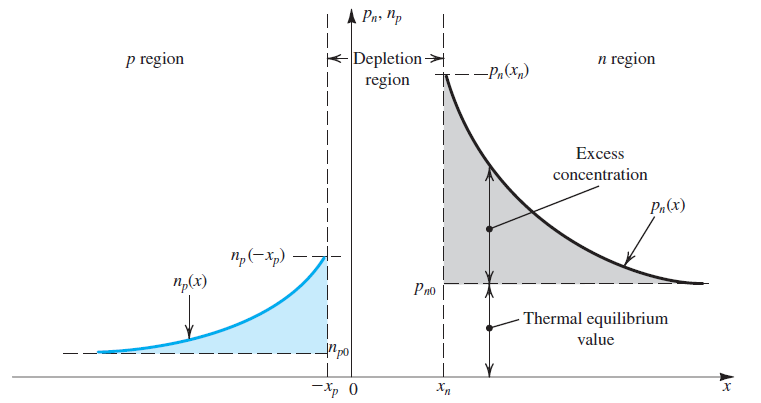
\includegraphics[scale=0.6]{Electronica/pn_f5.png}
\end{figure}

Que al reemplazar por la expresión de la concentración se llega a  

\begin{equation*}
J_p (x) = q \left( \frac{D_p}{L_p} \right) p_{n0} \left( e^{V/V_T} - 1 \right) e^{-(x-x_n)/L_p}
\end{equation*}

Como se espera, $J_p$ alxcanza su máximo en $x=x_n$

\begin{equation}
J_p (x_n) q \left( \frac{D_p}{L_p} \right) p_{n0} \left( e^{V/V_T} - 1 \right) 
\label{eq_densidadCorrienteDifusionHuecos}
\end{equation}

y decae exponencialmente para \(x > x_n\), a medida que los huecos minoritarios se recombinan con los electrones mayoritarios. Sin embargo, esta recombinación significa que los electrones mayoritarios tendrán que ser repuestos por una corriente que inyecte electrones desde el circuito externo hacia la región n de la unión. Este último componente de corriente tiene la misma dirección que la corriente de huecos (porque los electrones que se mueven de derecha a izquierda dan lugar a una corriente en la dirección de izquierda a derecha). Se deduce que a medida que \(J_p(x)\) disminuye, el componente de corriente de electrones aumenta exactamente en la misma cantidad, haciendo que la corriente total en el material n sea constante en el valor dado por la Ecuación \ref{eq_densidadCorrienteDifusionHuecos}.

Un desarrollo exactamente paralelo se puede aplicar a los electrones que son inyectados desde la región n a la región p, resultando en una corriente de difusión de electrones dada por una simple adaptación de la Ecuación \ref{eq_densidadCorrienteDifusionHuecos}.

\begin{equation*}
J_n(-x_p) = q \left( \frac{D_n}{L_n} \right) n_{p0} \left( e^{V/VT} - 1 \right)
\end{equation*}

Ahora, aunque las corrientes en las Ecuaciones anteriores se encuentran en los dos bordes de la región de agotamiento, sus valores no cambian en la región de agotamiento. Por lo tanto, podemos descartar los descriptores de ubicación \(x_n\) y \(-x_p\). Al sumar las dos densidades de corriente y multiplicarlas por el área de la unión A, obtenemos la corriente total I

\begin{eqnarray*}
I &=& A (J_p + J_n) \\
I &=& A q \left( \frac{D_P}{L_P} p_{n0} + \frac{D_n}{L_n} n_{p0} \right) \left( e^{V/V_T} - 1\right)
\end{eqnarray*}

Sustituyendo $p_{n0}=n_i^2/N_D$ y  $n_{p0}=n_i^2/N_A$,

\begin{equation*}
I = A q n_i^2 \left( \frac{D_n}{L_p N_D} + \frac{D_n}{L_n N_A} \right) \left( e^{V/V_T} - 1\right)
\end{equation*}

De esta ecuación observamos que para un V negativo (polarización inversa) con una magnitud de unas pocas veces \(V_T\) (25.9 mV), el término exponencial se vuelve esencialmente cero, y la corriente a través de la unión se vuelve negativa y constante. De nuestra descripción cualitativa en la Sección 3.5.1, sabemos que esta corriente debe ser \(I_S\). Así que,

\begin{equation}
I = I_s \left( e^{V/V_T} - 1 \right)
\label{eqVoltajeCorrienteDiodo}
\end{equation}

donde

\begin{equation*}
I_S = A q n_i^2 \left( \frac{D_n}{L_p N_D} + \frac{D_n}{L_n N_A} \right)
\end{equation*}

\begin{figure}[H]
    \centering
    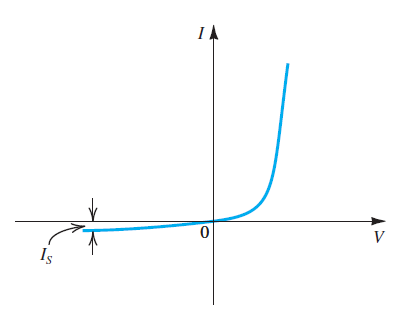
\includegraphics[scale=0.6]{Electronica/pn_f6.png}
    \caption{Curva Corriente Voltaje del diodo}
    \label{fig_curva_ID_Diodo}
\end{figure}

La Figura \ref{fig_curva_ID_Diodo} muestra la característica I–V de la unión pn (Ec. \ref{eqVoltajeCorrienteDiodo}). Observe que en la dirección inversa, la corriente se satura a un valor igual a \(-I_S\). Por esta razón, a \(I_S\) se le da el nombre de corriente de saturación. De la Ec. (\ref{eqVoltajeCorrienteDiodo}) vemos que \(I_S\) es directamente proporcional al área transversal A de la unión. Así, otro nombre para \(I_S\), que preferimos usar en este libro, es la corriente de escala de unión. Los valores típicos para \(I_S\), para uniones de varias áreas, varían de \(10^{-18} A\) a \(10^{-12} A\).

Además de ser proporcional al área de unión A, la expresión para \(I_S\) en la ecuación inmediatamente anterior indica que \(I_S\) es proporcional a \(n^2i\), que es una función muy fuerte de la temperatura.

\paragraph*{Ruptura en inverso}

La descripción del funcionamiento de la unión pn en la dirección inversa y la relación I-V de la unión en la Ec. \ref{eqVoltajeCorrienteDiodo}, indica que a un voltaje de polarización inversa -V, con \( V \gg VT \), la corriente inversa que fluye a través de la unión es aproximadamente igual a \( I_S \) y, por lo tanto, es muy pequeña. Sin embargo, a medida que se aumenta la magnitud del voltaje de polarización inversa V, se alcanza un valor en el que fluye una corriente inversa muy grande como se muestra en la Fig. \ref{fig_rupturaInversaCorrienteUnionPN} Observe que cuando V alcanza el valor \( V_Z \), el dramático aumento en la corriente inversa va acompañado de un pequeño aumento en el voltaje inverso; es decir, el voltaje inverso a través de la unión permanece muy cerca del valor \( V_Z \). El fenómeno que ocurre en \( V = V_Z \) es conocido como ruptura de la unión. No es un fenómeno destructivo. Es decir, la unión pn puede operarse repetidamente en la región de ruptura sin un efecto permanente en sus características. Sin embargo, esto se basa en la suposición de que la magnitud de la corriente de ruptura inversa está limitada por el circuito externo a un valor "seguro". El valor "seguro" es aquel que da como resultado la limitación de la potencia disipada en la unión a un nivel seguro y admisible.

Hay dos posibles mecanismos para la ruptura de la unión pn: el efecto Zener y el efecto avalancha. Si una unión pn se rompe con un voltaje de ruptura \( V_Z < 5 \) V, el mecanismo de ruptura suele ser el efecto Zener. La ruptura avalancha ocurre cuando \( V_Z \) es mayor que aproximadamente 7 V. Para las uniones que se rompen entre 5 V y 7 V, el mecanismo de ruptura puede ser ya sea el efecto Zener o el efecto avalancha o una combinación de los dos.

La ruptura Zener ocurre cuando el campo eléctrico en la capa de agotamiento aumenta hasta el punto de romper enlaces covalentes y generar pares electrón-hueco. Los electrones generados de esta manera serán arrastrados por el campo eléctrico hacia el lado n y los huecos hacia el lado p. Por lo tanto, estos electrones y huecos constituyen una corriente inversa a través de la unión. Una vez que comienza el efecto Zener, se pueden generar un gran número de portadores con un aumento negligible en el voltaje de la unión. Por lo tanto, la corriente inversa en la región de ruptura será grande y su valor debe ser determinado por el circuito externo, mientras que el voltaje inverso que aparece entre los terminales del diodo permanecerá cerca del voltaje de ruptura especificado \( V_Z \).

\begin{figure}
    \centering
    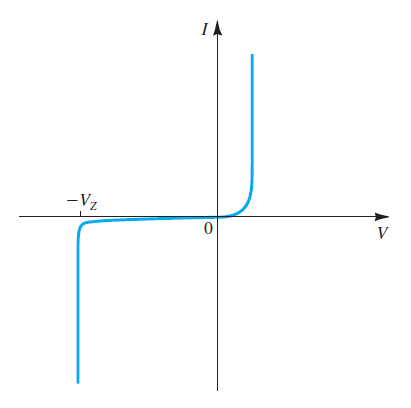
\includegraphics[scale=0.6]{Electronica/diodo_f1.png}
    \caption{Curva I-V de la unión pn mostrando el incremento repentino de corriente inversa en la región de ruptura}
    \label{fig_rupturaInversaCorrienteUnionPN}
\end{figure}

El otro mecanismo de ruptura, la ruptura avalancha, ocurre cuando los portadores minoritarios que cruzan la región de agotamiento bajo la influencia del campo eléctrico ganan suficiente energía cinética para poder romper enlaces covalentes en átomos con los que colisionan. Los portadores liberados por este proceso pueden tener suficiente energía para poder hacer que otros portadores sean liberados en otra colisión ionizante. Este proceso se repite al estilo de una avalancha, con el resultado de que se crean muchos portadores que pueden soportar cualquier valor de corriente inversa, según lo determine el circuito externo, con un cambio negligible en la caída de voltaje a través de la unión.

Como se verá en el capítulo siguiente, algunos diodos de unión pn están fabricados específicamente para operar en la región de ruptura, donde se aprovecha el voltaje casi constante \( V_Z \).


\subsubsection{Efectos capacitivos en la unión pn}

Hay dos mecanismos de almacenamiento de carga en la unión pn. Uno está asociado con la carga almacenada en la región de agotamiento, y el otro está asociado con la carga de portadores minoritarios almacenada en los materiales n y p como resultado de los perfiles de concentración establecidos por la inyección de portadores. Mientras que el primero es más fácil de ver cuando la unión pn está polarizada en inverso, el segundo está en efecto solo cuando la unión está polarizada en directo.

\paragraph*{Capacitancia de unión o de deplexión}

Cuando una unión $pn$ se polariza en inverso con un voltaje $V_R$, la carga almacenada en ambos lados de la región de agotamiento está dada por 

\begin{equation*}
Q_J = A \sqrt{2 \epsilon_s q \left( \frac{N_A N_D}{N_A + N_D} \right) \left( V_0 + V_R \right)}
\end{equation*}

si $\alpha = A \sqrt{2 \epsilon_s q \frac{N_A N_D}{N_A + N_D}}$, 

\begin{equation*}
Q_J = \alpha \sqrt{\left( V_0 + V_R \right)}
\end{equation*}

Así, \( Q_J \) está relacionado de manera no lineal con \( V_R \), como se muestra en la Figura \ref{fig_CargaQjEnFunciondelVoltajeInverso}. Esta relación no lineal hace que sea difícil definir una capacitancia que tenga en cuenta la necesidad de cambiar \( Q_J \) siempre que \( V_R \) sea cambiado. Sin embargo, podemos suponer que la unión está operando en un punto como Q, como se indica en la Figura \ref{fig_CargaQjEnFunciondelVoltajeInverso}, y definir una capacitancia \( C_j \) que relacione el cambio en la carga \( Q_J \) con un cambio en la tensión \( V_R \).

\begin{equation*}
C_j = \left. \frac{d Q_J}{d V_R}\right|_{V_R = V_Q}
\end{equation*}

\begin{figure}[H]
    \centering
    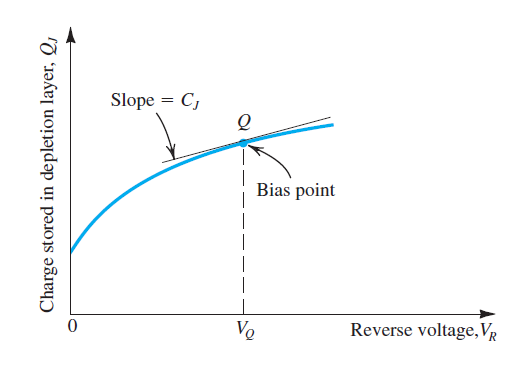
\includegraphics[scale=0.6]{Electronica/pn_f7.png}
    \caption{Carga en los lados de la zona de agotamiento en función del voltaje inverso.}
    \label{fig_CargaQjEnFunciondelVoltajeInverso}
\end{figure}

Este enfoque de capacitancia incremental resulta ser bastante útil en el diseño de circuitos electrónicos, como se verá más adelante.
Se tiene, entonces

\begin{equation*}
C_J = \frac{\alpha}{2 \sqrt{V_0 + V_R}}
\end{equation*}

Cuando la tensión en inverso es igual a cero, se tiene entonces

\begin{equation*}
C_{j0} = \frac{\alpha}{2 \sqrt{V_0}}
\end{equation*}

así, la expresión para $C_j$ queda

\begin{equation*}
C_j = \frac{C_{j0}}{\sqrt{1+ \frac{V_R}{V_0}}}
\end{equation*}

Y de otra forma, $C_{j0}$ está dado por

\begin{equation*}
C_{j0} = A \sqrt{\left( \frac{\epsilon_s q}{2} \right)\left( \frac{N_A N_D}{N_A + N_D} \right)\left( \frac{1}{V_0} \right)}
\end{equation*}

Antes de dejar el tema de la capacitancia en la región de agotamiento o la capacitancia de la unión, señalamos que en la unión pn que hemos estado estudiando, la concentración de dopaje se cambia abruptamente en la frontera de la unión. A tal unión se le conoce como una unión abrupta. Hay otro tipo de unión pn en la cual la concentración de portadores se cambia gradualmente de un lado de la unión al otro. Para permitir tal unión graduada, la fórmula para la capacitancia de la unión se puede escribir en la forma más general.

\begin{equation*}
C_j = \frac{C_{j0}}{\left( 1 + \frac{V_R}{V_0} \right)^m}
\end{equation*}

donde \( m \) es una constante llamada coeficiente de graduación, cuyo valor varía de 1/3 a 1/2 dependiendo de la manera en que la concentración cambia desde el lado p al lado n.

\paragraph*{Capacitancia de difusión}

Considérese una unión $pn$ polarizada en directo. En estado estacionario, se establecen distribuciones de portadores minoritarios en los materiales p y n, como se muestra en la figura anterior. Así, se almacena una cierta cantidad de carga de portadores minoritarios en exceso en cada una de las regiones a granel p y n (fuera de la región de agotamiento). Si el voltaje terminal \( V \) cambia, esta carga tendrá que cambiar antes de que se logre un nuevo estado estacionario. Este fenómeno de almacenamiento de carga da lugar a otro efecto capacitivo, claramente diferente de aquel debido al almacenamiento de carga en la región de agotamiento.
Para calcular la carga de portadores minoritarios en exceso, consulte la Figura 3.12. La carga de huecos en exceso almacenada en la región n se puede encontrar a partir del área sombreada bajo la exponencial de la siguiente manera:

\begin{eqnarray*}
Q_p &=& A q \times \text{ área sombreada bajo la curva } p_n(x) \\
&=& a Q \left[ p_n(x_n) - p_{n0} \right] L_p
\end{eqnarray*}

Sustituyendo por $p_n(x_n) = p_{n0} \left( e ^{\frac{V}{V_T}} - 1 \right)$ permite expresar $Q_p$ como

\begin{equation*}
Q_p = \frac{L_p^2}{D_p} I_p
\end{equation*}

el factor $\frac{L_p^2}{D_p}$ es un parámetro que tiene la unidad de segundos, por lo que es un tiempo $\tau_p$ quedando 

\begin{equation*}
Q_p = \tau_p I_p
\end{equation*}

La constante de tiempo \(\tau_p\) es conocida como el tiempo de vida de los portadores minoritarios en exceso (huecos). Es el tiempo promedio que tarda un hueco inyectado en la región n en recombinarse con un electrón mayoritario. Esta definición de \(\tau_p\) implica que toda la carga \(Q_p\) desaparece y tiene que ser repuesta cada \(\tau_p\) segundos. La corriente que logra la reposición es \(I_p = Q_p/\tau_p\). \\

Una relación similar a la de la Ecuación (3.52) se puede desarrollar para la carga de electrones almacenada en la región p,
\[ Q_n = \tau_n I_n \]
donde \( \tau_n \) es el tiempo de vida del electrón en la región p. La carga total de portadores minoritarios en exceso se puede obtener sumando \( Q_p \) y \( Q_n \),
\[ Q = \tau_p I_p + \tau_n I_n \]
Esta carga se puede expresar en términos de la corriente del diodo \( I = I_p + I_n \) como
\[ Q = \tau_T I \]
donde \( \tau_T \) se llama el tiempo medio de tránsito de la unión. Obviamente, \( \tau_T \) está relacionado con \( \tau_p \) y \( \tau_n \). Además, para la mayoría de los dispositivos prácticos, un lado de la unión está mucho más dopado que el otro. Por ejemplo, si \( N_A \gg N_D \), se puede demostrar que \( I_p \gg I_n \), \( I \approx I_p \), \( Q_p \gg Q_n \), \( Q \approx Q_p \), y por lo tanto \( \tau_T \approx \tau_p \).
Para pequeños cambios alrededor de un punto de polarización, podemos definir una capacitancia de difusión incremental \( C_d \) como

\begin{equation*}
C_d = \frac{d Q}{d V}
\end{equation*}

\begin{equation*}
C_d = \left( \frac{\tau_T}{V_T} \right) I
\end{equation*}

donde $I$ es la corriente de polarización directa. Note que $C_d$ es directamente proporcional a la corriente en directo y por tanto es tan pequeño que puede ser despreciada cuando el diodo está polarizado en inverso. También importante notar que para obtener un valor de $C_d$ pequeño, es necesario hacer$\tau_T$ pequeño; lo cual es un requerimiento muy importante para que una juntura pn sea diseñada para altas frecuencias.

\section{El diodo} \label{SeccionDiodo}

En los Capítulos anteriores, se han tratado casi en su totalidad con circuitos lineales; cualquier no linealidad, como la introducida por la saturación de la salida del amplificador, fue tratada como un problema a ser resuelto por el diseñador del circuito. Sin embargo, hay muchas otras funciones de procesamiento de señales que solo pueden ser implementadas por circuitos no lineales. Ejemplos de esto incluyen la generación de voltajes de corriente continua a partir de la fuente de alimentación de corriente alterna, y la generación de señales de diversas formas de onda (por ejemplo, sinusoides, ondas cuadradas, pulsos). Además, los circuitos lógicos y de memoria digitales constituyen una clase especial de circuitos no lineales.

El elemento de circuito no lineal más simple y fundamental es el diodo. Al igual que una resistencia, el diodo tiene dos terminales; pero a diferencia de la resistencia, que tiene una relación lineal (en línea recta) entre la corriente que fluye a través de ella y el voltaje que aparece en ella, el diodo tiene una característica i–v no lineal.

Esta sección se ocupa del estudio de los diodos. Para entender la esencia de la función del diodo, comenzamos con un elemento ficticio, el diodo ideal. Luego presentamos el diodo de unión de silicio, explicamos sus características terminales y proporcionamos técnicas para el análisis de los circuitos de diodos. La última tarea implica el importante tema de la modelización de dispositivos. Nuestro estudio de la modelización de las características del diodo sentará las bases para nuestro estudio de la modelización de la operación del transistor en los próximos tres capítulos.

De las muchas aplicaciones de los diodos, su uso en el diseño de rectificadores (que convierten de ca a dc) es el más común. Por lo tanto, estudiaremos los circuitos rectificadores con cierto detalle y examinaremos brevemente una serie de otras aplicaciones de diodos.

El diodo de unión no es más que la unión pn que estudiamos en la sección \ref{subSeccionUnionPN}, y la mayor parte de este capítulo se ocupa del estudio de los diodos de unión pn de silicio. En la última sección, sin embargo, consideramos brevemente algunos tipos de diodos especializados, incluyendo el fotodiodo y el diodo emisor de luz.

\subsection{El diodo ideal} \label{sSubSeccionDiodoIdeal}

\subsubsection{Característica corriente-tensión}

El diodo ideal es considerado el elemento no lineal fundamental en los circuitos. Tiene dos terminales y su símbolo y características se muestran en la figura \ref{fig_diodoIdeal}. Si se aplica una tensión negativa al diodo, no fluye corriente y se comporta como un circuito abierto, estando en un estado llamado "corte" o simplemente apagado. Esto se conoce como polarización inversa.

Por otro lado, si se aplica una corriente positiva, no hay caída de tensión en el diodo y se comporta como un cortocircuito, pasando cualquier corriente sin caída de tensión. Esto se llama polarización directa y el diodo está "encendido".

Es importante que el circuito externo limite la corriente directa y la tensión inversa a valores predeterminados. Se presentan dos ejemplos de circuitos diodo que ilustran este punto. En un circuito, el diodo conduce y la corriente es de 10 mA, mientras que en el otro, el diodo está cortado y no hay corriente.

Los terminales del diodo se denominan ánodo y cátodo. La característica i-v del diodo ideal, que conduce en una dirección y no en la otra, explica su símbolo en forma de flecha.

La característica i-v del diodo ideal es altamente no lineal y se describe como "lineal por tramos". Si un dispositivo con esta característica se utiliza en una aplicación de manera que la señal solo se desplace a lo largo de uno de los segmentos lineales, puede considerarse un elemento de circuito lineal en ese contexto particular. Sin embargo, si las señales pasan uno o más de los puntos de quiebre, el análisis lineal ya no es posible.

\begin{figure}[H]
    \centering
    \includegraphics[scale=0.6]{Electronica/Diodo_F1.png}
    \caption{Diodo ideal con sus equivalentes con polarizaciones directa e inversa}
    \label{fig_diodoIdeal}
\end{figure}

\subsubsection{Una aplicación simple: Rectificador}


\begin{figure}[H]
    \centering
    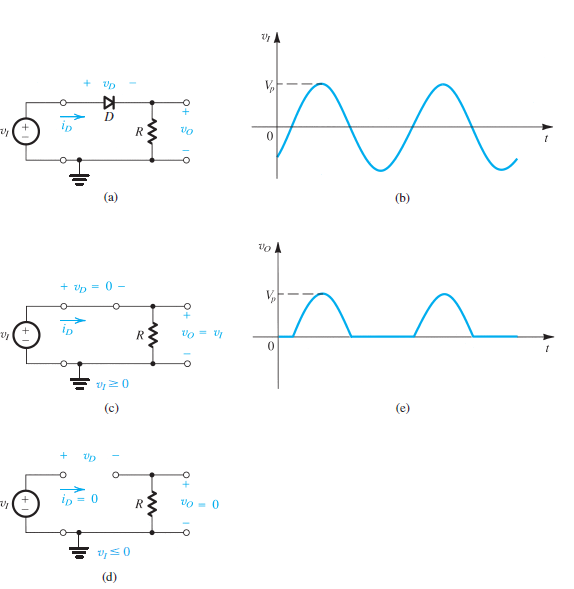
\includegraphics[scale=0.6]{Electronica/diodo_f2.png}
    \caption{Circuito rectificador y la forma de onda de salida}
    \label{fig_rectificadorIdeal}
\end{figure}

Una aplicación fundamental del diodo, que aprovecha su curva i-v severamente no lineal, es el circuito rectificador. El circuito consiste en la conexión en serie de un diodo D y una resistencia R. Si la tensión de entrada \( vI \) es la sinusoidal mostrada, y se supone que el diodo es ideal, el funcionamiento es el siguiente:


\begin{itemize}
    \item Durante los semiciclos positivos de la sinusoidal, la tensión positiva \( v_I \) provocará que la corriente fluya a través del diodo en su dirección directa, haciendo que la tensión del diodo \( v_D \) sea muy pequeña, idealmente cero. En este caso, el circuito equivalente tendrá la salida \( v_O \) igual a la tensión de entrada \( v_I \).
    \item Durante los semiciclos negativos de \( v_I \), el diodo no conducirá, y la tensión de salida \( v_O \) será cero.
\end{itemize}


Así, la tensión de salida tendrá la forma de onda mostrada, que es unidireccional y tiene un valor promedio finito o un componente de continua. A diferencia de \( v_I \), que alterna en polaridad y tiene un valor promedio cero, \( v_0 \) convierte la señal alterna en continua. Por lo tanto, el circuito rectifica la señal y se llama rectificador, y puede ser utilizado para generar corriente continua a partir de corriente alterna.

\subsection{Características terminales del diodo de unión}

La implementación más común del diodo utiliza una unión pn. Ya hemos estudiado la física de la unión pn y derivado su característica $i - v$ en la sección \ref{subSeccionUnionPN}. Que la unión pn se use para implementar la función de diodo no debería sorprendernos: la unión pn puede conducir una corriente sustancial en la dirección directa y casi ninguna corriente en la dirección inversa. En esta sección, estudiamos en detalle la característica $i - v$ del diodo de unión pn para prepararnos para las aplicaciones de circuitos de diodos.

\begin{figure}[H]
    \centering
    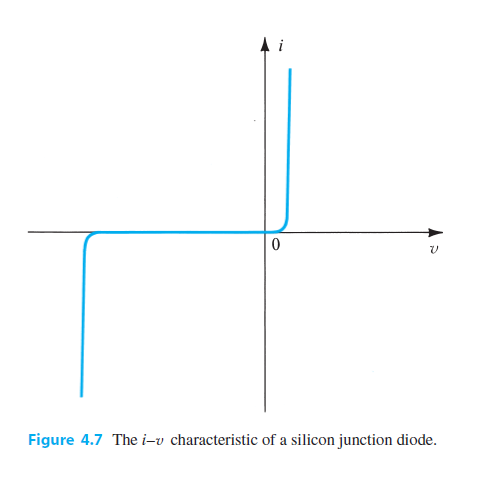
\includegraphics[scale=0.6]{Electronica/diodo_f3.png}
    \caption{Curva característica del diodo de union pn}
    \label{fig_curvaCaracteristicaDiodo}
\end{figure}

La característica i–v de un diodo de unión de silicio se muestra en la figura \ref{fig_curvaCaracteristicaDiodo} La misma característica se muestra en la \ref{fig_curvaCaracteristicaDiodoExp} con algunas escalas expandidas y otras comprimidas para revelar detalles. Obsérvese que los cambios de escala han resultado en la aparente discontinuidad en el origen.

Como se indica, la curva característica consta de tres regiones distintas:
1. La región de polarización directa, determinada por \( v > 0 \)
2. La región de polarización inversa, determinada por \( v < 0 \)
3. La región de ruptura, determinada por \( v < -V_{ZK} \)

Estas tres regiones de operación se describen en las siguientes secciones.

\begin{figure}[H]
    \centering
    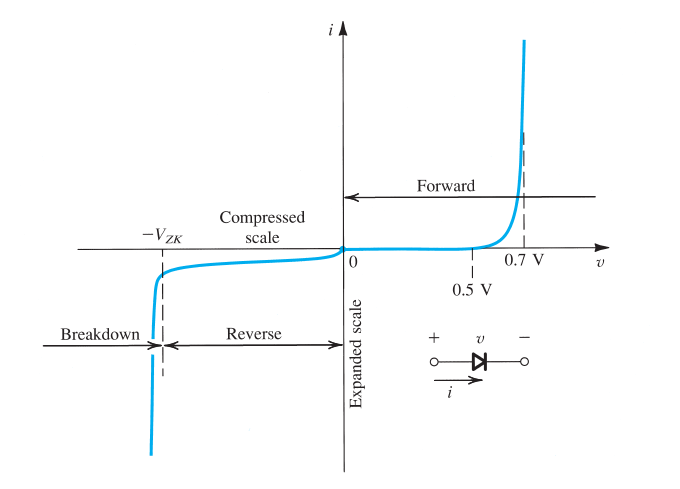
\includegraphics[scale=0.6]{Electronica/diodo_f4.png}
    \caption{Relación i-v del diodo de union pn con escalas expandidas para ver detalles}
    \label{fig_curvaCaracteristicaDiodoExp}
\end{figure}

\subsubsection{Región de polarización directa}





La región de polarización directa, o simplemente la región directa, se alcanza cuando la tensión en los terminales \( v \) es positiva. En la región directa, la relación i–v está aproximada de cerca por:

\begin{equation}
i = I_S (e^{\frac{v}{V_T}}-1)
\label{eq_CorrienteDiodo}
\end{equation}

En esta ecuación, \( I_S \) es una constante para un diodo dado a una temperatura dada. Se proporcionó una fórmula para \( I_S \) en términos de los parámetros físicos del diodo y la temperatura. La corriente \( I_S \) generalmente se llama la corriente de saturación (por razones que se harán evidentes en breve). Otro nombre para \( I_S \), y uno que ocasionalmente usaremos, es la corriente de escala. Este nombre surge del hecho de que \( I_S \) es directamente proporcional al área de la sección transversal del diodo. Así, el doblar el área de la unión resulta en un diodo con el doble del valor de \( I_S \) y, como indica la ecuación del diodo, el doble del valor de la corriente \( i \) para una tensión directa \( v \) dada. Para los diodos "de pequeña señal", que son diodos de pequeño tamaño destinados a aplicaciones de baja potencia, \( I_S \) es del orden de \( 10^{-15} \, \text{A} \). Sin embargo, el valor de \( I_S \) es una función muy fuerte de la temperatura. Como regla general, \( I_S \) se duplica en valor por cada aumento de temperatura de \( 5\, ^\circ\text{C} \).

La tensión \( V_T \) en la Ec. \ref{eq_CorrienteDiodo}  es una constante llamada la tensión térmica y se da por:

\[ V_T = \frac{kT}{q} \]

Aquí, \( k \) es la constante de Boltzmann, \( T \) es la temperatura absoluta en kelvins, y \( q \) es la carga del electrón. \\

Por lo tanto, a temperatura ambiente (20°C), el valor de \( V_T \) es 25.3 mV. En el análisis rápido aproximado de circuitos, usaremos \( V_T \approx 25 \, \text{mV} \) a temperatura ambiente.

Para una corriente apreciable \( i \) en la dirección directa, específicamente para \( i \gg I_S \), la Ecuación (4.1) se puede aproximar por la relación exponencial:

\begin{equation}
i \approx I_S \, e^{\frac{v}{V_T}}
\label{eq_Corriente_i_diodoAproximado}
\end{equation}
Esta aproximación es útil en el análisis de circuitos de diodos en la región de polarización directa, donde la corriente fluye fácilmente a través del diodo. La relación anterior también se puede expresar en forma logarítmica como:

\[ v \approx V_T \ln \left( \frac{i}{I_S} \right) \]

La relación exponencial entre la corriente \( i \) y el voltaje \( v \) se mantiene a lo largo de muchos órdenes de magnitud de corriente (se puede encontrar un rango de hasta siete órdenes de magnitud, es decir, un factor de \( 10^7 \)). Esta es una propiedad bastante notable de los diodos de unión, que también se encuentra en los transistores de unión bipolar y que ha sido explotada en muchas aplicaciones interesantes.

Consideremos la relación de polarización directa \( i-v \) en la Ecuación \ref{eq_Corriente_i_diodoAproximado} y evaluemos la corriente \( I_1 \) correspondiente a un voltaje de diodo \( V_1 \):

\[ I_1 = I_S  e^{\frac{V_1}{V_T}} \]

Ahora, consideramos la corriente para un voltage $V_2$

\[ I_2 = I_S  e^{\frac{V_2}{V_T}} \]

Combinando estas ecuaciones obtenemos 

\begin{equation*}
\frac{I_2}{I_1} = e^{\frac{V_2-V_1}{V_T}}
\end{equation*}

\begin{equation*}
V_2-V_1 = V_T \ln{\frac{I_2}{I_1}}
\end{equation*}

O en términos de logaritmo en base 10:

\begin{equation*}
V_2-V_1 = 2.3 V_T \log{\frac{I_2}{I_1}}
\end{equation*}

Esta ecuación indica que, para un cambio de una década (factor de 10) en la corriente, la caída de voltaje en el diodo cambia por \(2.3V_T\), que es aproximadamente 60 mV. Esto también sugiere que la relación i-v del diodo se representa más convenientemente en un gráfico semilogarítmico. Utilizando el eje vertical lineal para \( v \) y el eje horizontal logarítmico para \( i \), se obtiene una línea recta con una pendiente de 60 mV por década de corriente.

Una mirada a la característica i-v en la región de polarización directa (Fig. \ref{fig_curvaCaracteristicaDiodoExp}) revela que la corriente es insignificante para \( v \) menor a aproximadamente 0.5 V. Este valor suele denominarse voltaje de corte. Sin embargo, debe enfatizarse que este aparente umbral en la característica es simplemente una consecuencia de la relación exponencial. Otra consecuencia de esta relación es el rápido aumento de \( i \). Por lo tanto, para un diodo "completamente conductor", la caída de voltaje se encuentra en un rango estrecho, aproximadamente 0.6 V a 0.8 V. Esto da lugar a un "modelo" simple para el diodo, donde se asume que un diodo conductor tiene aproximadamente una caída de 0.7 V en él. Los diodos con diferentes calificaciones de corriente (es decir, áreas diferentes y, por ende, diferentes \( I_S \)) exhibirán la caída de 0.7 V en diferentes corrientes. Por ejemplo, un diodo de pequeña señal puede considerarse que tiene una caída de 0.7 V en \( i = 1 \, \text{mA} \), mientras que un diodo de mayor potencia puede tener una caída de 0.7 V en \( i = 1\, \text{A} \). Estudiaremos los temas del análisis de circuitos de diodos y los modelos de diodos en la siguiente sección.

\begin{figure}[H]
    \centering
    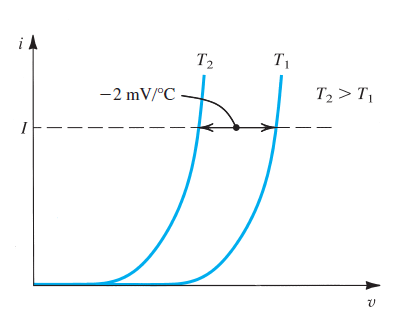
\includegraphics[scale=0.6]{Electronica/diodo_f5.png}
    \caption{Dependencia de la temperatura de la característica en directo. Con corriente constante, la caída de tensión decae aprox $2mV$ por cada grado de aumento de temperatura}
    \label{fig_dependenciaDiodoaTemperatura}
\end{figure}


Dado que tanto \( I_S \) como \( V_T \) son funciones de la temperatura, la característica i-v en la región de polarización directa varía con la temperatura, como se ilustra en la Fig \ref{fig_dependenciaDiodoaTemperatura} A una corriente de diodo constante dada, la caída de voltaje a través del diodo disminuye aproximadamente 2 mV por cada aumento de 1°C en la temperatura.

Este cambio en el voltaje del diodo con la temperatura ha sido aprovechado en el diseño de termómetros electrónicos.

\subsubsection{Región de polarización inversa}

La región de polarización inversa en el funcionamiento de un diodo se produce cuando el voltaje del diodo \( v \) es negativo. La Ecuación \ref{eq_CorrienteDiodo} predice que si \( v \) es negativo y su magnitud es unas pocas veces mayor que \( V_T \) (25 mV), el término exponencial se vuelve insignificante en comparación con la unidad, y la corriente del diodo se convierte en:
\[ i \approx -I_S \]
Es decir, la corriente en la dirección inversa es constante e igual a \( I_S \). Esta constancia es la razón detrás del término corriente de saturación.

Los diodos reales muestran corrientes inversas que, aunque son bastante pequeñas, son mucho mayores que \( I_S \). Por ejemplo, un diodo de pequeña señal cuyo \( I_S \) está en el orden de \( 10^{-14} \, \text{A} \) a \( 10^{-15} \, \text{A} \) podría mostrar una corriente inversa en el orden de 1 nA. La corriente inversa también aumenta un poco con el aumento de la magnitud del voltaje inverso. Debido a la magnitud muy pequeña de la corriente, estos detalles no son claramente evidentes en la característica i-v del diodo de la Fig. \ref{fig_curvaCaracteristicaDiodoExp}.

Gran parte de la corriente inversa se debe a los efectos de fuga. Estas corrientes de fuga son proporcionales al área de la unión, al igual que \( I_S \). Sin embargo, su dependencia de la temperatura es diferente de la de \( I_S \). Así, mientras que \( I_S \) se duplica por cada aumento de 5°C en la temperatura, la regla general para la dependencia de la temperatura de la corriente inversa es que se duplica por cada aumento de 10°C en la temperatura.

\subsubsection{Región de ruptura}

La tercera región distinta de operación del diodo es la región de ruptura, que se puede identificar fácilmente en la característica i-v del diodo en la Fig. \ref{fig_curvaCaracteristicaDiodoExp}. Se entra en la región de ruptura cuando la magnitud del voltaje inverso supera un valor umbral específico para el diodo particular, llamado voltaje de ruptura. Este es el voltaje en la "rodilla" de la curva i-v en la Fig. \ref{fig_curvaCaracteristicaDiodoExp} y se denota \( V_{ZK} \), donde el subíndice Z significa zener y K denota rodilla.

Como se puede ver en la Fig. \ref{fig_curvaCaracteristicaDiodoExp}, en la región de ruptura, la corriente inversa aumenta rápidamente, siendo el aumento asociado en la caída de voltaje muy pequeño. La ruptura del diodo normalmente no es destructiva, siempre que la potencia disipada en el diodo esté limitada por la circuitería externa a un nivel "seguro". Este valor seguro normalmente se especifica en las hojas de datos del dispositivo. Por lo tanto, es necesario limitar la corriente inversa en la región de ruptura a un valor consistente con la disipación de potencia permisible.

El hecho de que la característica i-v del diodo en ruptura sea casi una línea vertical permite que se utilice en la regulación de voltaje. La región de ruptura se explora en dispositivos como los diodos Zener, que se utilizan específicamente para mantener un voltaje constante en una parte de un circuito, independientemente de las fluctuaciones en la tensión de entrada o la carga. La capacidad de mantener un voltaje constante incluso cuando la corriente cambia rápidamente hace que los diodos Zener sean valiosos en aplicaciones como la regulación de voltaje y la protección contra sobretensiones.

\subsection{Modelamiento de la características en polarización directa}

\begin{figure}[H]
    \centering
    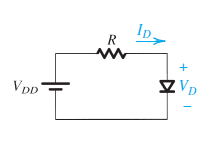
\includegraphics{Electronica/diodo_f6.png}
    \caption{Circuito simple para ilustrar el análisis de circuitos con diodos}
    \label{fig_circuitoSimpleDiodoRes}
\end{figure}

Habiendo estudiado las características terminales del diodo, ahora estamos listos para considerar el análisis de circuitos que emplean diodos en conducción directa. La Figura \ref{fig_circuitoSimpleDiodoRes} muestra un circuito de este tipo. Consiste en una fuente de CC \( V_{DD} \), una resistencia \( R \), y un diodo. Queremos analizar este circuito para determinar el voltaje del diodo \( V_D \) y la corriente \( I_D \). Para ayudar en nuestro análisis, necesitamos representar el diodo con un modelo.

Existen varios modelos de diodos, de los cuales ahora conocemos dos: el modelo de diodo ideal y el modelo exponencial. En la siguiente discusión, evaluaremos la idoneidad de estos dos modelos en diversas situaciones de análisis. Además, desarrollaremos y comentaremos otros modelos. Este material, además de ser útil en el análisis y diseño de circuitos de diodos, establece una base para la modelización del funcionamiento del transistor que estudiaremos en los próximos tres capítulos.

\subsubsection{Modelo exponencial}

El modelo exponencial ofrece una descripción precisa del funcionamiento de un diodo en la región de polarización directa, pero su naturaleza no lineal lo hace complejo de usar.

Si analizamos un circuito que incluye una fuente de tensión \( V_{DD} \), una resistencia \( R \), y un diodo, y suponemos que \( V_{DD} \) es mayor que aproximadamente 0.5 V, la corriente del diodo será significativamente mayor que la corriente de saturación \( I_S \). Esto nos permite utilizar la relación exponencial:

\[ I_D = I_S e^{V_D/V_T} \]

Adicionalmente, aplicando la ley de Kirchhoff en este circuito, se obtiene:

\[ I_D = \frac{V_{DD}-V_D}{R} \]

Con estas dos ecuaciones, y conociendo el valor de \( I_S \), podemos resolver el sistema para encontrar \( I_D \) y \( V_D \). Esto se puede hacer mediante análisis gráfico o un proceso iterativo.


\subsubsection{Necesidad de un análisis rápido}

El procedimiento de análisis iterativo es simple y ofrece resultados precisos después de dos o tres iteraciones. Sin embargo, hay situaciones en las que el esfuerzo y el tiempo requeridos pueden ser mayores de lo justificable. 

Cuando se está diseñando un circuito relativamente complejo a mano, es necesario realizar un análisis rápido para evaluar varias posibilidades antes de decidirse por un diseño de circuito adecuado. Para acelerar el proceso de análisis, es posible que se tenga que conformar con resultados menos precisos. Esto no suele ser un problema, ya que se puede posponer el análisis más preciso hasta obtener un diseño final o casi final.

El análisis preciso del diseño casi final se puede realizar con la ayuda de un programa de análisis de circuitos por computadora, como SPICE. Los resultados de tal análisis luego pueden usarse para refinar o "ajustar" aún más el diseño.

Para agilizar el proceso de análisis, es necesario encontrar un modelo más simple para la característica de polarización directa del diodo.

\subsubsection{Modelo de caída constante de voltaje}

\begin{figure}[H]
    \centering
    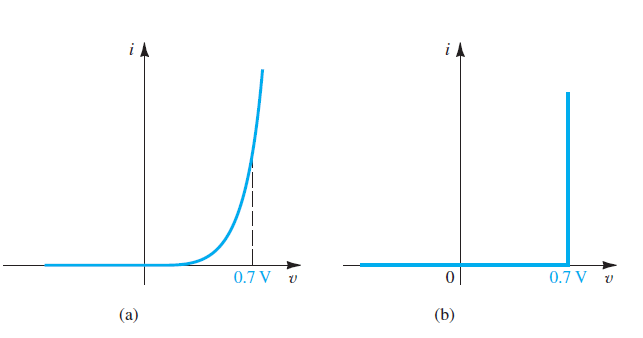
\includegraphics[scale=0.6]{Electronica/diodo_f7.png}
    \caption{Modelo aproximado del diodo}
    \label{fig_ModeloDiodoAproximado}
\end{figure}


El modelo de diodo más simple y ampliamente utilizado es el modelo de caída de voltaje constante. Este modelo se basa en la observación de que un diodo en conducción directa tiene una caída de voltaje que varía en un rango relativamente estrecho, digamos, de 0.6 a 0.8 V. El modelo asume que este voltaje es constante en un valor, por ejemplo, 0.7 V.

El modelo de caída de voltaje constante es el que se utiliza con más frecuencia en las fases iniciales de análisis y diseño. Esto es especialmente cierto si en estas etapas no se tiene información detallada sobre las características del diodo, lo cual suele ser el caso (Fig. \ref{fig_ModeloDiodoAproximado}).

\subsubsection{Modelo ideal}

En aplicaciones que involucran voltajes mucho mayores que la caída de voltaje del diodo (0.6 V - 0.8 V), podemos ignorar completamente la caída de voltaje del diodo al calcular la corriente del diodo. Esto resulta en el modelo de diodo ideal, que estudiamos en una sección anterior. Sin embargo, con casi ningún trabajo adicional, el modelo de caída de 0.7 V ofrece resultados mucho más realistas. Cabe destacar, sin embargo, que la mayor utilidad del modelo de diodo ideal radica en determinar cuáles diodos están encendidos y cuáles apagados en un circuito con múltiples diodos.

\subsubsection{Modelo de pequeña señal}

\begin{figure}
    \centering
    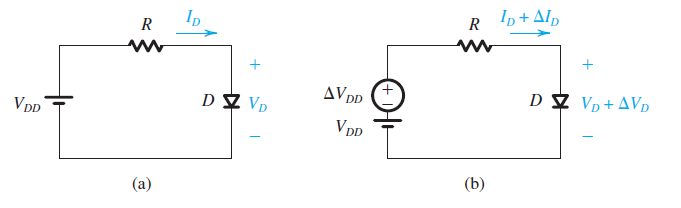
\includegraphics[scale=0.6]{Electronica/diodo_f8.png}
    \caption{(a) Circuito simple de diodo; (b) situación que resulta en cambiar $V_{DD}$ por $\Delta V_{DD}$}
    \label{fig_CircuitoSimpleParaPequenasenal}
\end{figure}

Consideremos la situación en la Figura \ref{fig_CircuitoSimpleParaPequenasenal}(a), donde un voltaje de corriente continua \( V_{DD} \) establece una corriente continua \( I_D \) a través de la combinación en serie de una resistencia \( R \) y un diodo \( D \). El voltaje resultante del diodo se denota como \( V_D \). Como se mencionó anteriormente, los valores de \( I_D \) y \( V_D \) se pueden obtener resolviendo el circuito usando la característica exponencial del diodo o, mucho más rápidamente, se pueden encontrar valores aproximados utilizando el modelo de caída de voltaje constante del diodo.

A continuación, consideremos la situación en la que \( V_{DD} \) sufre un pequeño cambio \( \Delta V_{DD} \), como se muestra en la Figura \ref{fig_CircuitoSimpleParaPequenasenal}(b). Como se indica, la corriente \( I_D \) cambia en un incremento \( \Delta I_D \), y el voltaje del diodo \( V_D \) cambia en un incremento \( \Delta V_D \). Queremos encontrar una forma rápida de determinar los valores de estos cambios incrementales. Para ello, desarrollamos un modelo de "señal pequeña" para el diodo.

\begin{figure}
    \centering
    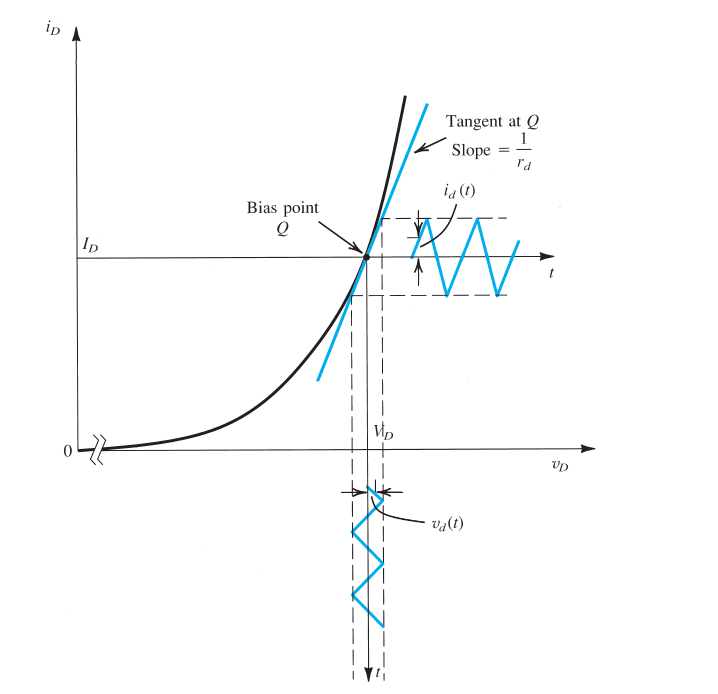
\includegraphics[scale=0.6]{Electronica/diodo_f9.png}
    \caption{Desarrollo de modelo de pequeña señal del diodo}
    \label{fig_ModeloPequenaSenalDiodo}
\end{figure}

Aquí, la palabra "señal" enfatiza que, en general, \( \Delta V_{DD} \) puede ser una cantidad variable en el tiempo. El calificador "pequeño" indica que este modelo de diodo solo se aplica cuando \( \Delta V_D \) se mantiene suficientemente pequeño, con "suficientemente" que se cuantificará en breve.

Para desarrollar el modelo de señal pequeña del diodo, refiérase a la Figura '\ref{fig_ModeloPequenaSenalDiodo}. Expresamos el voltaje a través del diodo como la suma del voltaje de corriente continua \( V_D \) y la señal variable en el tiempo \( v_d(t) \).

\begin{equation*}
v_D (t) = V_D + v_d (t)
\end{equation*}

Correspondientemente la corriente total instantánea es

\begin{equation*}
i_D = I_S e^{\frac{v_D}{V_T}}
\end{equation*}
Al hacer las ustituciones adecuadas se tiene que 

\begin{eqnarray*}
i_D &=& I_S e^{\frac{V_D + v_d (t)}{V_T}} \\
i_D &=& I_S e^{\frac{V_D}{V_T}}e^{\frac{v_d (t)}{V_T}} \\
\end{eqnarray*}

En ausencia de la señal \( v_d(t) \), el voltaje del diodo es igual a \( V_D \), y la corriente del diodo es

\begin{equation*}
I_D = I_S e^{\frac{V_D}{V_T}}
\end{equation*}

Por tanto la corriente $i_D (t)$ se expresa como

\begin{equation*}
i_D (t) = I_D e^{\frac{V_D}{V_T}}
\end{equation*}

Ahora, si la amplitud de la señal $v_d(t)$ es lo suficientemente pequeña tal que
\begin{equation*}
\frac{v_d}{V_T} \ll 1
\end{equation*}

Entonces se puede realizar una expansión en series de potencia de la exponencial de la corriente $i_D(t)$ y solo considerar las dos primeras sumas

\begin{equation*}
i_D (t) \approx I_D \left( 1 + \frac{v_d}{V_T}\right)
\end{equation*}

Esta es la aproximación de señal pequeña. Es válida para señales cuyas amplitudes son menores de aproximadamente $5 mV$. Partiendo de 

\begin{equation*}
i_D (t) = I_D  + \frac{I_D}{V_T} v_d
\end{equation*}

Por lo tanto, superpuesto en la corriente continua \( I_D \), tenemos un componente de corriente de señal directamente proporcional al voltaje de señal \( v_d \). Es decir,

\begin{equation*}
i_D = I_D + i_d
\end{equation*}

donde $i_d = \frac{I_D}{V_T} v_d$. La cantidad que relaciona la corriente de señal \( i_d \) con el voltaje de señal \( v_d \) tiene las dimensiones de conductancia, mhos (S), y se llama conductancia de señal pequeña del diodo. El inverso de este parámetro es la resistencia incremental del diodo o resistencia de señal pequeña, \( r_d \),

\begin{equation*}
r_d = \frac{V_T}{I_D}
\end{equation*}

 Observa que el valor de \( r_d \) es inversamente proporcional a la corriente de polarización \( I_D \).

Se puede obtener una comprensión adicional de la aproximación de señal pequeña y del modelo de diodo de señal pequeña considerando nuevamente la construcción gráfica en la Fig. 4.14. Aquí se ve que el diodo está operando en un punto de polarización en continua Q caracterizado por el voltaje en continua \( V_D \) y la corriente en continua correspondiente \( I_D \). Superpuesto en \( V_D \) tenemos una señal \( v_d(t) \), que se supone (arbitrariamente) tiene una forma de onda triangular.

Es fácil ver que usar la aproximación de señal pequeña es equivalente a suponer que la amplitud de la señal es lo suficientemente pequeña como para que la excursión a lo largo de la curva i-v se limite a un segmento casi lineal y corto. La pendiente de este segmento, que es igual a la pendiente de la tangente a la curva i-v en el punto de operación Q, es igual a la conductancia de señal pequeña.

Se anima al lector a probar que la pendiente de la curva i-v en \( i = I_D \) es igual a \( I_D / V_T \), que es \( 1 / r_d \); es decir,

\begin{equation*}
r_d = \frac{1}{\left[ \frac{\partial i_D}{\partial v_D} \right]}
\end{equation*}

A partir de lo anterior, concluimos que superpuestas a las cantidades \( V_D \) e \( I_D \) que definen el punto de polarización en continua, o punto de reposo, del diodo estarán las cantidades de señal pequeña \( v_d(t) \) e \( i_d(t) \), que están relacionadas por la resistencia de señal pequeña del diodo \( r_d \) evaluada en el punto de polarización. Por lo tanto, el análisis de señal pequeña se puede realizar por separado del análisis de polarización en continua, una gran comodidad que resulta de la linealización de las características del diodo inherente en la aproximación de señal pequeña. Específicamente, después de que se realiza el análisis en continua, se obtiene el circuito equivalente de señal pequeña eliminando todas las fuentes en continua (es decir, cortocircuitando las fuentes de voltaje en continua y dejando en circuito abierto las fuentes de corriente en continua) y reemplazando el diodo por su resistencia de señal pequeña. Así, para el circuito en la Fig. \ref{fig_circuitoSimpleDiodoRes}(b), el análisis en continua se obtiene utilizando el circuito en la Fig. \ref{fig_circuitoSimpleDiodoRes}(a), mientras que las cantidades incrementales \( \Delta I_D \) y \( \Delta V_D \) se pueden determinar utilizando el circuito equivalente de señal pequeña mostrado en la Fig. \ref{fig_circuitoPequenaSenal}.

\begin{figure}[H]
    \centering
    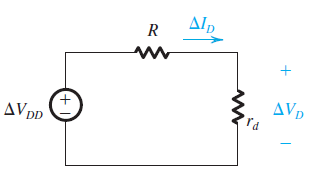
\includegraphics[scale=0.6]{Electronica/diodo_f10.png}
    \caption{Circuito para obtener las cantidades incrementales de corriente y voltaje para la pequeña señal}
    \label{fig_circuitoPequenaSenal}
\end{figure}

\subsubsection{Uso de la caída de voltaje como regulación de tensión}

Una de las aplicaciones que pueden tener los diodos, es en la regulación de tensión. Un regulador de tensión es un circuito cukyo propósito es proveer una tensión DC constante entre sus terminales de salida. Para un regulador se requiere que la salida de tensión permanezca lo más constante posible sin importar cambios en la impedancia de carga o de la tensión de alimentación del mismo regulador. Un diodo en directo puede servir como un regulador de tensión ya que el voltaje puede permanecer relativamente constante a $0.7V$. 

\paragraph{Ejemplo} Considere el siguiente circuito

\begin{figure}[H]
    \centering
    \begin{circuitikz}[american,scale=0.5, transform shape]
        \draw[-{Latex[scale=1.5]}] (0,4) -- (0,5) node[midway, left, font=\fontsize{16}{16}\selectfont] {$10V$};
    % Resistor
        \draw (0,4) to[R] (0,2) node[above=10mm,right=2mm, font=\fontsize{16}{12}\selectfont] {$R=1k\Omega$};
        \node at (0,2) [circle,fill,inner sep=2.5pt]{};
        \draw (0,2) to (2,2);
        \node at (2,2) [circle,fill,inner sep=2.5pt]{};
        \node at (3,2) [circle,fill,inner sep=2.5pt]{};
        % \node at (3,1) [above, font=\fontsize{16}{12}\selectfont] {+};
        % \node at (3,1) [below, font=\fontsize{16}{12}\selectfont] {-};
        \node at (2,1) [font=\fontsize{18}{12}\selectfont] {\( V_0 \)};
        % Three diodes in series
        \draw (3,2) to (4,2);
        \draw (4,2) to[R] (4,-4) node[above=30mm,right=2mm, font=\fontsize{16}{12}\selectfont] {$R_L=1k\Omega$};;
        \draw (0,2)  to[D] (0,0);
        \draw (0,0)  to[D] (0,-2);
        \draw (0,-2)  to[D] (0,-4);
        \draw (0,-4) node[ground, scale=1.5]{};
        \draw (4,-4) node[ground, scale=1.5]{};
    \end{circuitikz}
\end{figure}

Un arreglo de tres diodos se usan para proveer una tensión constante de 2.1V a la carga. Se requiere calcular el porcentaje de cambio de la tensión regulada causada por a) un cambio de $\pm 10\%$ de la tensión de alimentación y b) una carga de $1k\Omega$


\paragraph{Solución}

La corriente nominal sin carga del circuito es

\begin{equation*}
I = \frac{10-2.1}{1000} = 7.9mA
\end{equation*}

De este modo, cada diodo tendrá una resistencia incremental de 

\begin{equation*}
r_d = \frac{V_T}{I} = 3.2\Omega
\end{equation*}

Los tres diodos en serie tendrán una resistencia incremental de $9.6 \Omega$. \\
Esta resistencia, junto con la resistencia R, forma un divisor que servirá para determinar el cambio de tensión en el diodo

\begin{equation*}
\Delta v = 1V
\end{equation*}

\begin{equation*}
\Delta v_o = 3.2\frac{2V}{1000+3.2} =  19mV \text{pico a pico} 
\end{equation*}

Eso significa que cuando la tensión de alimentación varía $pm1V$ ($\pm 10\%$), la tensión en los diodos va a variar $\pm9.5mV$ o lo que es equivalente $\pm0.5\%$

Si se le conecta una resistencia de carga al circuito de $1k\omega$ habrá una corriente de aproximadamente $2.1mA$, esa corriente se disminuye de los diodos, resultando en una disminución del voltaje en los diodos que está dada por

\begin{equation*}
\Delta v_o = -2.1mA \times 9.6 \Omega = -20mV
\end{equation*}

\subsection{Operación en la región de ruptura en inverso: diodo zener}

La curva $i-v$ del diodo se vuelve muy empinada (ver fig \ref{fig_curvaCaracteristicaDiodo}) en la región de rompimiento muestra que en esta región el voltaje también muestra un valor semi constante y esto puede ser utilizado para regulación de tensión. De hecho, resulta que esta es una aplicación importante de los diodos que operan en la región de ruptura inversa, y se fabrican diodos especiales para operar específicamente en la región de ruptura. Estos diodos se llaman diodos de ruptura o, más comúnmente, como se señaló anteriormente, diodos zener.

En la operación normal del zener la corriente fluye hacia el cátodo, el cual es positivo con respecto al ánodo, así $I_z$ y $V_Z$ tienen valores positivos

\begin{figure}[H]
    \centering
    \begin{circuitikz}[american,scale=0.5, transform shape]
        \draw (0,0)  to[zD] (0,-2);  % Zener diode
        \node at (1,0) [font=\fontsize{18}{12}\selectfont] {\( + \)};
        \node at (1,-1) [font=\fontsize{18}{12}\selectfont] {\( V_Z \)};
        \node at (1,-2) [font=\fontsize{18}{12}\selectfont] {\( - \)};
        \draw[-latex, thick] (-1,0) -- (-1,-1) node[midway, left=3mm, font=\fontsize{18}{12}\selectfont] {\( I_Z \)};
    \end{circuitikz}
\end{figure}

\subsubsection{Modelamiento del diodo zener}

De la figura Fig \ref{FigDiodoZenerCurvaCaracteristica} podemos observar que para corrientes mayores a la corriente rodilla $I_{ZK}$, la curva característica es casi una línea recta. Los fabricantes de diodos usualmente especifican el voltaje de zener a una corriente de prueba específica $I_{ZT}$. A medida que la corriente en el diodo de desvía de $I_{ZT}$, el voltaje también variará. La figura muestra que el cambio correspondiente $\Delta I$ produce un cambio del voltaje $\Delta V$ dado por 

\begin{equation*}
\Delta V = r_Z \Delta I
\end{equation*}

donde $r_Z$ es en inverso de la pendiente de la curva cuasi-lineal $i-v$ en el punto Q. $r_Z$ es la resistencia incremental del zener en el punto de operación. 

\begin{figure}[H]
    \centering
    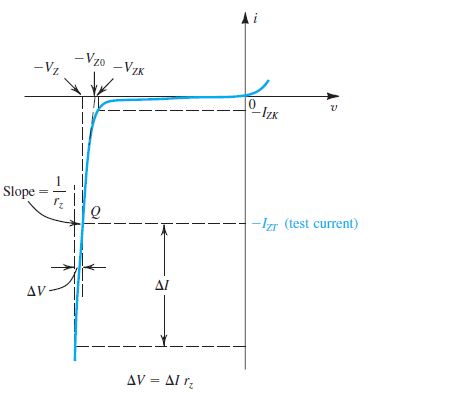
\includegraphics[scale=0.6]{Electronica/zener/zener_f1.png}
    \caption{Curva Característica del diodo zener}
    \label{FigDiodoZenerCurvaCaracteristica}
\end{figure}

Típicamente el valor de $r_Z$ está en el rango de unos pocos a decenas de ohmios. Evidentemente mientras más pequeño es $r_Z$, el voltaje permanecerá más constante a variaciones de la corriente, y el comportamiento será más cercano al ideal. EL modelo del zener puede aproximarse a una fuente de tensión en serie con la resistencia $r_Z$. El valor de la fuente es $V_{Z0}$, que es el punto en el que la pendiente $1/r_Z$ cruza con el eje $v$. En la práctica, $V_{Z0}\approx V_{ZK}$.

\begin{equation*}
V_Z = V_{Z0} + r_Z I_Z
\end{equation*}

\subsubsection{Uso como regulador de tensión}

\begin{figure}[H]
    \centering
    \begin{circuitikz}

        % fuente de tensión
        \draw (0,2) node[vcc](VCC){$V_{CC}={10}{V}$};
        \draw (0,2) to [R=$R\eq0.5k\Omega$] (0,0);

        \node at (0,0) [circ]{};
        \draw (0,0) to (2,0);
        \node at (1,0) [ocirc]{};
        \draw (2,0) to [R=$R_L$] (2,-2);
        \draw (2,-2) node[ground]{};
         
        \draw (0,-2) to [zzD] (0,0);
        \draw (0,-2) node[ground]{};
    \end{circuitikz}
    \begin{circuitikz}[american]

        % fuente de tensión
        \draw (0,2) node[vcc](VCC){$V_{CC}={10}{V}$};
        \draw (0,2) to [R=$R\eq0.5k\Omega$] (0,0);
        
        \node at (0,0) [circ]{};
        \draw (0,0) to (2,0);
        \node at (1,0) [ocirc]{};
        \node at (1,-1) [above] {\( V_o \)};
        \node at (1,-0) [below] {\( + \)};
        
        \draw (0,-2) to [R=$r_Z$] (0,0);
        \draw (0,-3) to [battery2=$V_{Z0}$] (0,-2);
        \draw (0,-3) node[ground]{};

        % rama carga
        \draw (2,0) to [R=$R_L$] (2,-3);
        \draw (2,-3) node[ground]{};
         
        % \draw (0,-2) to [zzD] (0,0);
        
    \end{circuitikz}
\end{figure}

Utilicemos el circuito anterior como ejemplo de uso del zener como regulador de tensión. El voltaje $V_Z = 6.8V$ a $I_Z=5mA$, $r_Z=20 \omega$ e $I_{ZK}=0.2 mA$. La tensión de alimentación es de $10V$ pero con una variación de $\pm1V$.

\begin{enumerate}
    \item Encontrar $V_o$ sin carga y con $V_{CC}$ en su valor nominal.
    \item Encontrar el cambio en $V_o$ que resulta del cambio de $\pm1V$ en $V_{CC}$. Note que $\left( \Delta V_o / \Delta V_{CC} \right)$, usualmente expresado como $\frac{\text{mV}}{V}$, es conocido como regulación de línea.
    \item Encuentre el cambio de $V_o$ resultante de conectar una carga $R_L$ por la que fluye una corriente $I_L=10\text{mA}$, y encuentre la regulación de carga $\left( \Delta V_o / I_L \right)$ dada en $\frac{\text{mV}}{\text{mA}}$.
    \item Encuentre el cambio de $V_o$ cuando $R_L=2 k\Omega$
    \item Encuentre el cambio de $V_o$ cuando $R_L=0.5 k\Omega$
    \item ¿Cuál es el valor mínimo de $R_L$ para el cual el diodo sigue operando en la región zener?
\end{enumerate}

\paragraph{Solución}

\begin{enumerate}
    \item Si no hay resistencia de carga, el voltaje $V_{Z0}$ es

    $V_{Z0} = V_Z - r_ZI_Z = 6.8 - (20)(0.005)=6.7 \text{V}$
    
    la corriente que pasa por \(R\) es:

    \(I_Z = \frac{V_{CC}-V_{Z0}}{R+r_Z} = \frac{10-6.7}{500+20} = 6.34 \text{mA}\)

    entonces, $V_o = V_{R_Z}+V_{Z0} = 6.7+20(0.00634)=6.83 V$

    \item Si la tensión cambia $\pm1V$, entonces la variación de la salida es

    \begin{equation*}
        \Delta V_o = r_Z \left( \frac{\Delta V_{CC}}{r_Z + R} \right) = \pm 38.2 \text{mV}
    \end{equation*}

    que es la regulación de línea.

    \item Si se conecta una carga que consume $1\text{mA}$, se asume que la tensión en el diodo no cambia ($V_Z = 6.8$V); entonces la corriente en la resistencia $R$ es la misma ($6.4$mA), por tanto la corriente del zener disminuirá $1$mA, y el cambio de $V_o$ será

    \begin{equation*}
        \Delta V_o = r_Z \Delta I_{Z} = -20 \text{mV}
    \end{equation*}

    Por tanto la regulación es de $-20$ mV/mA

    \item Si la resistencia de carga es $R_L=2 k\Omega$, entonces, la corriente será de aproximadamente 

    \begin{equation*}
        \frac{6.8}{2000} = 3.4\text{mA}
    \end{equation*}

    Entonces la corriente en el zener disminuye $\Delta I_Z = -3.4\text{mA}$. Y el cambio en el voltaje será 

    \begin{equation*}
        \Delta V_Z = r_Z \Delta I_Z = 20(-3.4\times 10^{-3}) = -68 \text{mV}
    \end{equation*}

    \item Si la carga baja a $0.5 k\Omega$, entonces la corriente sería de 
    
    \begin{equation*}
        \frac{6.8}{500} = 13.6\text{mA}
    \end{equation*}

    Pero esto no puede ser, porque la corriente de la resistencia $R$ debe ser $I=6.4$mA, entonces el diodo tendría que tener una corriente positiva en directo, y ya no estaría en la región de ruptura inversa. En este escenario el diodo dejaria de conducir, y la tensión en la salida estaría dada por la división de tensión entre $R$ t $R_L$.

    \begin{equation*}
        V_o = R_L \left( \frac{V_{CC}}{R+R_L} \right) = 500 \left( \frac{10}{1000} \right) = 5 \text{V}
    \end{equation*}

    \item Para que el diodo siga en la región de zener, el valór más bajo de $I_Z$ es de $0.2$mA. entonces la corriente máxima por la carga será 

    \begin{equation*}
        6.4-0.2 = 6.2\text{mA}
    \end{equation*}
 
    Así que la resistencia de carga será  $R_{L_{min}}=1.09 k\Omega$

    
    
\end{enumerate}